





% Template for PLoS
% Version 1.0 January 2009
%
% To compile to pdf, run:
% latex plos.template
% bibtex plos.template
% latex plos.template
% latex plos.template
% dvipdf plos.template

\documentclass[10pt]{article}

% amsmath package, useful for mathematical formulas
\usepackage{amsmath}
% amssymb package, useful for mathematical symbols
\usepackage{amssymb}

% graphicx package, useful for including eps and pdf graphics
% include graphics with the command \inputgraphics
\usepackage{graphicx}
\usepackage{lscape}

% cite package, to clean up citations in the main text. Do not remove.
\usepackage{cite}

\usepackage{color} 

% Use doublespacing - comment out for single spacing
\usepackage{setspace} 
\doublespacing


% Text layout
\topmargin 0cm
\oddsidemargin 0.5cm
\evensidemargin 0.5cm
\textwidth 16cm 
\textheight 21cm

% Bold the 'Figure #' in the caption and separate it with a period
% Captions will be left justified
\usepackage[labelfont=bf,labelsep=period,justification=raggedright]{caption}

%load my own packages (not PLoS template)
\usepackage{textcomp, fixltx2e}
\usepackage{fullpage, lscape}
\usepackage{lineno}

% Use the PLoS provided bibtex style
\bibliographystyle{plos2009}

% Remove brackets from numbering in List of References
\makeatletter
\renewcommand{\@biblabel}[1]{\quad#1.}
\makeatother


% Leave date blank
\date{}

\pagestyle{myheadings}
%% ** EDIT HERE **


%% ** EDIT HERE **
%% PLEASE INCLUDE ALL MACROS BELOW

%% END MACROS SECTION

\usepackage{Sweave}
\begin{document}
\Sconcordance{concordance:ligpaper.tex:ligpaper.Rnw:%
1}
\Sconcordance{concordance:ligpaper.tex:./rscripts.Rnw:ofs 1:%
18 1 42 1 13 1 6}
\Sconcordance{concordance:ligpaper.tex:ligpaper.Rnw:ofs 5:%
3 70 1 1 0 155 1}
\Sconcordance{concordance:ligpaper.tex:./fig_mb.Rnw:ofs 232:%
93}
\Sconcordance{concordance:ligpaper.tex:ligpaper.Rnw:ofs 233:%
230 12 1}
\Sconcordance{concordance:ligpaper.tex:./metaprot2.Rnw:ofs 246:%
56}
\Sconcordance{concordance:ligpaper.tex:ligpaper.Rnw:ofs 247:%
244 10 1}
\Sconcordance{concordance:ligpaper.tex:./fig_f2b.Rnw:ofs 258:%
186}
\Sconcordance{concordance:ligpaper.tex:ligpaper.Rnw:ofs 259:%
256 10 1}
\Sconcordance{concordance:ligpaper.tex:./fig_lci.Rnw:ofs 270:%
15}
\Sconcordance{concordance:ligpaper.tex:ligpaper.Rnw:ofs 271:%
268 11 1}
\Sconcordance{concordance:ligpaper.tex:./fig_degr.Rnw:ofs 283:%
83}
\Sconcordance{concordance:ligpaper.tex:ligpaper.Rnw:ofs 284:%
281 10 1}
\Sconcordance{concordance:ligpaper.tex:./fig_graphcorr.Rnw:ofs 295:%
111}
\Sconcordance{concordance:ligpaper.tex:ligpaper.Rnw:ofs 296:%
293 14 1}
\Sconcordance{concordance:ligpaper.tex:./metaprot_plot.Rnw:ofs 311:%
89}
\Sconcordance{concordance:ligpaper.tex:ligpaper.Rnw:ofs 312:%
309 19 1 1 13 43 0 1 2 4 1 1 45 42 0 1 2 3 1 1 34 42 0 1 2 3 1 1 8 55 0 %
1 2 4 1}
\Sconcordance{concordance:ligpaper.tex:./fig_Psequestr.Rnw:ofs 536:%
101}
\Sconcordance{concordance:ligpaper.tex:ligpaper.Rnw:ofs 537:%
452 9 1}
\Sconcordance{concordance:ligpaper.tex:./fig_pyrpca.Rnw:ofs 547:%
11}
\Sconcordance{concordance:ligpaper.tex:ligpaper.Rnw:ofs 548:%
463 9 1}


% Title must be 150 characters or less
\begin{flushleft}
{\Large
\textbf{Litter nutrient contents controls extend of lignin decomposition via decomposer community composition in Beech litter }
}
\\
% Insert Author names, affiliations and corresponding author email.
% Insert Author names, affiliations and corresponding author email.
Lukas Kohl$^{1}$, % $^{3,\ast}$
Wolfgang Wanek$^{1}$, 
Katharina Keiblinger$^{2,3}$, 
Sonja Leitner$^{1,3}$, 
Maria Mooshammer$^{1}$, 
Ieda H\"ammerle$^{1}$, 
Lucia Fuchslueger$^{1}$, 
J\"org Schnecker$^{1}$, 
Thomas Schneider$^{4,5}$
Sandra Moll$^{7}$
Markus Gorfer$^{7,8}$
Joseph Strauss$^{7,8}$
Katharina Riedel$^{4,6}$
Leo Eberl$^{4,5}$
Sophie Zechmeister-Boltenstern$^{2,3}$, 
Andreas Richter$^{1}$,
\\
\bf{1} Department of Chemical Ecology and Ecosystem Research, University of Vienna, Althanstrasse 14, A-1090 Vienna, Austria
\\
\bf{2} Federal Research and Training Centre for Forests, Natural Hazards and Landscape, Department of Soil Biology, Seckendorff-Gudent-Weg 8, A-1131 Vienna, Austria
\\
\bf{3} Current address: Institute for Soil Science, University of Natural Resources and Life Sciences, Peter Jordan-Stra\ss e 82, A-1180, Vienna, Austria
\\
\bf{4} Institute of Plant Biology, University of Zurich, Winterthurerstrasse 190, CH-8057, Zurich, Switzerland
\\
\bf{5} Current address: Institute of Plant Biology, University of Zurich, Zollikerstrasse 107, CH-8008, Zurich, Switzerland
\\
\bf{6} Current address: Institute of Microbiology, Ernst-Moritz-Arndt University of Greifswald, Friedrich-Ludwig-Jahn-Strasse 15, D-17487 Greifswald, Germany
\\
\bf{7} Fungal Genetics and Genomics Unit, Department of Applied Genetics and Cell Biology, University of Natural Resources and Life Sciences, Konrad-Lorenz-Strasse 24, A-3430 Tulln, Austria
\\
\bf{8} AIT Austrian Institute of Technology GmbH, Bioresources Unit, Konrad-Lorenz-Strasse 24, A-3430 Tulln, Austria

$\ast$ E-mail: Corresponding author@institute.edu
\end{flushleft}

\newpage
% Please keep the abstract between 250 and 300 words
\section*{Abstract}

Lignin is a major component of plant litter and is considered highly resistant to decomposition. Carbohydrates, in contrast, are more easily degraded. We studied the decomposition rates of these two compound classes, and to which extent they are controlled by litter C:N:P stoichiometry. 

Herein we report results from a 15-months mesocosm experiment under controlled climatic conditions with beech litter of different N and P contents. Litter was sterilized and re-inoculated prior to the experiment to minimize differences in the initial microbial community, but study the effect of N and P contents on identical initial decomposer communities. Lignin and carbohydrate decomposition rates were determined by pyrolysis-GC/MS for 2 periods (0-6 months and 6-15 months), the composition of the microbial community was monitored via metaproteome analysis.

Different in litter nutrient contents led to the establishment of different decomposer communities. Fungi were dominant on all litter, but fungi:bacteria ratios were highest on high-nutrient litter, leading to a negative correlation between litter and microbial stoichiometry and high differences between litter and microbial C:N and C:P ratios on nutrient poor litter.

Rates of lignin decomposition were highly variable during the first six months, ranging from insignificant amounts decomposed to decomposition at bulk C mineralization rates. Between 6 and 15 months, lignin was degraded at bulk mass loss rates independent of the litter nutrient contents, however, different lignin contents aquired within the initial 6 months remained in place. Early lignin degradation rates were highest in litter with low fungi:bacteria ratios, and were correlated to differences between litter and microbial stoichiometry (C:P$_{litter : microbial}$ and C:P$_{litter : microbial}$). Lignin degrading communities were enriched in $\gamma$-proteobacteria after 6 months incubation.

Our results indicate that - contradicting common models - significant amounts of lignin were be degraded during early decomposition in low nutrient litter. We demonstrate that litter quality profoundly affects the lignin decomposition via the composition of the decomposer community. Even though bacterial biomass is enriched in N and P, communities low nutrient litter were enriched in bacteria. This led to higher differences between litter and microbial stoichiomety, a possible control over lignin degradation during early decomposition. 

\linenumbers %not from the template: start line numbers here.
\newpage%not in original layout
\input{introduction}
% Results and Discussion can be combined.
\section*{Results}
\subsection*{Initial litter chemistry}
Initial litter chemistry of the four sites (Achenkirch, AK, Klausenleopoldsdorf, KL, Ossiach, OS, Schottenwald, SW), measured 14 days after incubation, is presented in supplemental table \ref{initstoech}. C:N ratios varied between 41:1 and 58:1 and C:P ratios between 700:1 and 1300:1, while N:P ratios ranged between 15:1 and 30:1. No significant changes occurred during litter incubation except a slight decrease of the C:N ratio (41.8:1 to 37.4:1) found in the most active litter type (SW) after 15 months. Fe concentrations were more than twice as high for OS (approx. 450 ppm) than for other litter types (approx. 200 ppm). Litter Mn also was highly variable between litter types, ranging between 170 and 2130 ppm. Changes of micro-nutrient concentrations during litter incubation were significant, but in all cases \textless 15\% of the initial concentration. In initial litter, lignin accounted for 28.9-31.2\% and carbohydrates for 25.9-29.2\% of the total peak area of all pyrolysis products.

\subsection*{Mass loss, respiration and soluble organic carbon}

Litter mass loss was not significant after 2 weeks and 3 months, and significant for 2 litter from two sites after 6 months. After 15 months, litter mass loss was significant for all collection sites, and ranged between 5 and 12 \% of the initial dry mass, and was strongly correlated to litter N content (R=0.794, p\textless 0.001). Detailed results were reported by \cite{Mooshammer2011}.

Highest respiration rates were measured at the first measurement after 14 days incubation (150-350 \textmu g CO$_2$-C d$^{-1}$ g$^{-1}$ litter-C), which dropped to 75 to 100 \textmu g CO$_2$-C d$^{-1}$ g$^{-1}$ litter-C after 3 months. After 6 and 15 months, respiration rates for AK and OS further decreased, while SW and KL showed a second maximum in respiration after 6 months (fig \ref{fig:enz}). Accumulated respiration was strongly correlated to litter mass loss after 15 months (r=0.738, p\textless 0.001, n=20).

Soluble organic carbon concentrations decreased between the first three harvests (14 days to 6 months), and strongly increased to 15 months (from 0.1 to 0.7 mg C g$^{-1}$  d.w. to 1.5 to 4 mg C g$^{-1}$ d.w. after 15 months, fig. \ref{fig:enz}). After 14 days and 3 months, the highest soluble organic C concentrations were found in SW litter followed by AK. Soluble organic C concentrations were weakly correlated with litter N content after 14 days (r=0.69, p\textless 0.001, n=20) and after 3 months (r = 0.65, p\textless 0.01, n=20), but strictly correlated after 6 months (r=0.85, p\textless 0.001, n=20) and 15 months (r=0.90, p\textless 0.001, n=20).

\subsubsection*{Potential enzyme activities}
Within each time point, all potential extracellular enzyme activities were correlated with litter N and actual respiration rates(all R\textgreater 0.8, p\textless 0.001, n=20). Cellulase activity increased from the first harvest onwards to 15 months, with a small depression after 6 months (Fig. \ref{fig:enz}), phenoloxidase and peroxidase activities reached their maximum between 3 and 6 months (fig. \ref{fig:enz}). For all enzymes and at all time points, SW showed the highest and AK the lowest activities. Differences between these two sites were more pronounced in cellulase activity (SW 10x higher than AK) than in oxidative enzymes (SW 4x higher). Conversely, the phenoloxidase/cellulase ratio was highest for AK and lowest for SW at all time points and decreased during litter decomposition (fig. \ref{fig:enz}).

\subsubsection*{Microbial biomass abundance and community composition}
Microbial biomass contents ranged from 0.5 to 6 mg C g$^{-1}$ d.w., 0.05 to 0.55 mg N g$^{-1}$ d.w. and 0.05 to 0.35 mg P g$^{-1}$ litter d.w (fig. \ref{fig:mb}). After an initial increase in microbial biomass, in KL and OS microbial biomass remained constant after 3 months while AK and SW showed further microbial biomass growth reaching a maximum of microbial C and N contents after 6 months (AK also for P). Microbial C:N ratios ranged between 6:1 and 18:1, C:P ratios between 8:1 and 35:1, and N:P ratios between 0.5:1 and 3.5:1 (fig. \ref{fig:mb}).

Microbial biomass was stoichiometrically homeostatic during the first 6 months (no or negative correlations between microbial C:N:P and litter C:N:P, see also \cite{Mooshammer2011}), but after 15 months (microbial C:N:P ratios were significantly and positively correlated to resource stoichiometry: R=0.53-0.64, all p\textless 0.002). The homeostatic regulation coefficients \cite{Sterner2002} were H\textsubscript{C:P}=1.68, H\textsubscript{C:N}=2.01, and H\textsubscript{N:P}=2.29 after 15 month incubation. Microbial C:N ratios after 3 and 6 months were within a tighly constrained range, 14.5:1 to 18.2:1 after 3 months and 6.9:1 to 9.0:1 after 6 months, but significantly different between the two sampling events. In contrast, microbial C:P and N:P ratios were less constrained, with the highest variance between litter from different sites after 3 months of incubation (fig. \ref{fig:mb}).

Metaproteome analysis yielded between 451 and 1113 (average 639) assigned spectra sample (one replicate per collection site after 14 days, 3, 6, and 15 months). Only spectra assigned to bacteria or fungi were used for community profiling. Fungal proteins were dominant in all litter types at all stages, but most prominent in SW and least pronounced in  AK. Fungi:bacteria (F:B) protein abundance ratios were highest after 14 days (5 to 12) and decreased during litter decomposition (1.7 to 3 after 15 months, see fig. \ref{fig:f2b}). The large initial differences in F:B ratios between litter from different sites decreased during decomposition. In addition, F:B ratios were measured on a DNA basis (qPCR) the results showing a similar pattern but with a much larger fungal DNA dominance (F:B ratios between 10-180). F:B ratios were highly correlated between protein- and log-transformed DNA-based estimates (r=0.785, p\textless 0.001, n=20).

Fungal communities were dominated by Ascomycetes, with smaller contributions by Basidiomycetes (<5\% of fungal protein).  Among the fungal classes found, Sordariomycetes and Eurotiomycetes were most abundant with further contributions of Dothideomycetes, Leothiomycetes and Saccharomycetes (fig. \ref{fig:metaprot_barplot}). Bacteria were dominated by Proteobacteria (mainly $\gamma$, declining, and $\alpha$- and $\beta$-Proteobacteria, increasing with litter decomposition) with minor contribution of Actinomycetes and Bacterioidetes (both increasing) and Thermotogae (decreasing, fig. \ref{fig:metaprot_barplot}).

\subsection*{Pyrolysis-GC/MS and Lignin content}
In total 128 pyrolysis products were detected, quantified, identified and assigned to their substances of origin (suppl. tab. \ref{tab:phprod} -\ref{tab:nprod}). We found only minor changes in the relative concentration of litter pyrolysis products during decomposition, and differences between sites were small but well preserved during decomposition. However, the high precision and reproducibility of pyrolysis GC/MS analysis of litter allowed tracing small changes in lignin and carbohydrate abundance during decomposition. Lignin-derived compounds made up between 29 and 31 \% relative peak area (TIC) in initial litter, and increased by up to 3 \%. The increase occured almost exclusively during the first 6 months. Carbohydrate-derived pyrolysis products accounted for 26 to 29 \% in initial litter and decreased by up to 2.6 \% within 15 months of incubation. The initial (pyrolysis-based) lignin:carbohydrate indices (LCI) were highly similar between litter from different collection sites, ranging between 0.517 and 0.533 (Fig. 4). During decomposition, the LCI increased by up to 9 \% of the initial value. The highest increase was found in SW litter, while LCI slightly decreased in AK litter. All significant changes in LCI  occurred within the first 6 months (fig. \ref{fig:lci}). As differences in lignin and carbohydrate contents between 0-3 and 3-6 months were not significant, we analyzed differences for two time intervals, i.e. between 0-6 months and 6-15 months.

During the first 6 months, between one and 6 \% of the initial lignin pool and between 4 and 17\% of the initial carbohydrate pool were degraded (Fig. \ref{fig:degr}). Lignin decomposition was highest in AK and KL litter, while microbial communities of KL, OS and SW litter decomposed carbohydrates faster. Lignin preference values (\% lignin decomposed : \%carbohydrates decomposed) were lowest in SW and highest in AK litter (Figure 5). In AK litter, lignin macromolecules were 50 \% more likely to be decomposed than carbohydrates, while in SW litter carbohydrates were 10 times more likely to be decomposed (fig. \ref{fig:degr}). Between 6 and 15 months, no further accumulation of lignin occurred. Lignin and carbohydrates were both degraded at the same rate and their relative concentrations remained constant between 6 and 15 months (fig. \ref{fig:degr}).

\subsection*{Correlations between lignin and carbohydrate decomposition and litter chemistry, microbial community and decomposition processes}

Relationships between lignin and carbohydrate degradation, litter chemistry, microbial biomass and decomposition processes were tested after 6 and 15 months (tables \ref{corrtable} and \ref{corrtable2}) including data presented by \cite{Mooshammer2011} and \cite{Leitner2011}. After 6 months, we found that the ratio of lignin/cellulose degradation was positively correlated with the ratio of phenoloxidase : cellulase (R=0.599, p=0.005, n=20) and peroxidase : cellulase (R=0.734 p\textless 0.001, n=20). Carbohydrate decomposition was positively correlated with litter N content, and negatively with litter C:N ratios and litter-microbial C:N imbalances. In contrast, lignin decomposition was negatively correlated to litter P, but positively with litter C:P and N:P ratios, and litter-microbial C:P and N:P imbalances (fig. \ref{fig:cor1}). After 15 months, the ratio of lignin : carbohydrate decomposition was no longer related to stoichiometry or elemental composition any more. Most interestingly, lignin and carbohydrate decomposition exhibited the same controls, being positively correlated to soluble organic C, litter N and litter P (table \ref{corrtable2}) between 6 and 15 months. Mass loss and accumulated respiration were positively correlated to lignin and carbohydrate decomposition (table \ref{corrtable2}), a pattern that we did not find for lignin decomposition in the early decomposition phase (table \ref{corrtable}). Protein abundance F:B ratios were negatively correlated to the ratios of lignin : cellulose decomposition and to LCI change during the first 6 months, pointing to bacterial engagement in lignin decomposition. In contrast, both lignin and carbohydrate decomposition rates, were positively correlated with F:B ratios after 15 months, pointing to fungal dominance of both lignin and carbohydrate decompostion. No correlation between F:B ratio and the ratio of lignin : cellulose decomposition was found in this later period (fig. \ref{fig:f2b}).


To asses the interaction between litter chemistry, microbial community and degradation processes, we conducted a correspondence analysis (CA) of the metaprotomen data (relative protein abundances, fig. \ref{fig:metaprotpca}). The results indicate that incubations time (i.e. succession) is the dominant factor controlling the microbial community, with samples collected at the first (14 days) and the last (15 month) sampling grouping closely together, while litter quality (i.e. elemental stoichiometry of litter collected at different sites) had a higher impact after 3 and 6 months. The first factor (CA 1), which explained 35.7 \% of the total variance, separates litter sampled after 15 months (positive values) from litter sampled earlier (negative values). Consequently, CA 1 was also positively correlated to incubation time and negatively to litter carbon content (i.e. decreasing C:N ratios during decomposition) . A number of bacterial taxa (Actinobacteria, Bacteroidetes, Alpha- and Betaproteobacteria), and two fungal classes (Leotiomycetes and Tremellomycetes) were positively correlated to CA1 i.e. increased in abundance towards 15 months, while Cyanobacteria, Epsilonproteobacteria and Saccharomycetes were negatively correlated. CA 2, which explained 26.0 \% variance, separated litter sampled within the first 6 months. Dothideomycetes and Sordariomycetes were positively and Gammaproteobacteria negatively correlated to this factor, which also correlated to the F:B protein abundance ratio. Litter collected 14 days after inoculation have the highest scores on CA 2, while sites with active lignin degradation within the first 6 months (AK, KL) have the most negative scores. The axis was furthermore correlated to the microbial biomass P content and C:P and N:P imbalances (and free NH\textsubscript{4}\textsuperscript{+}, not shown). For samples analyzed after 6 months, where direct comparison to lignin degradation rates was possible, significant correlations to CA 2 were found for lignin : carbohydrate degradation (r=-0.97, p=0.028), \% Lignin loss : \% Carbon loss (r=-0.96, p=0.040) and  LCI increase (r=0.973, p=0.027), even though the number of independent samples was very low (n=4). Differences in CA2 strongly decreased after 15 months, suggesting that the differences in the microbial community found within the first 6 months were siminished with succession of the decomposer community. Litter N and P contents were not correlated to either factor, although differences in resource quality evidently affected community composition after 3 and 6 months, as can be seen in the differences in the microbial communities as observed in CA 2. Correlation of CA factors with litter stoichiometry, and microbial stoichiometry, and the abundance of the analyzed taxa are provided in supplemental table \ref{catab}.
\section*{Discussion}

We used beech litter collected at different sites to study the effect of litter quality on decomposition. Differences in litter quality led to different mass loss rates, different extends of lignin accumulation during early decomposition, and the development of of different decomposer communities from a common inoculate. Our study was designed to investigate the effect of litter N and P, and we chose our collection sites to provide litter with different N and P contents. Positive correlations between litter N and bulk decomposition parametres like carbon mineralization rates and extracellular enzymatic activities indicate a N limitation. No such correlation was found for litter P contents. However, AK litter, which had low contents in both N and P, had a lower C mineralization rate than KL and OS, which were had lower contents of N or P, respectively, than AK, suggesting a co-limitation of both elements. The use of litter of a single species from different sites minimized differences in other 
litter traits, and eg. initial carbohydrate and lignin contents of all samples fell in a narrow range for litter from all sites. However, litter N and P contents are also proxies for other litter traits not directly measurable (e.g. leaf morphology), which resulted from the plant’s response to nutrient availability (e.g. for low P adaptation see \cite{Vence2003}). N and P were also demostrated to be correlated to a wide area of leaf traits in plants (ref\footnote{good ref for leaf economy spectrum needed!}), and leaf traits were successfully uised to predict litter decomposeability \cite{Cornelissen1997}. % a sentence of N & P fertilization vs. N & P variance in litter?

The composition of the microbial community changed with both by time (i.e. succession) and collection site (i.e. litter quality). While all samples measured were dominated by fungi,  fungi:bacteria ratios decreased over time and were higher in nutrient-rich litter than in nutrient-poor litter (SW >> AK). Our results contradicted the often-cited predictions that higher N and P contents would favor bacterial over fungal growth because bacterial biomass has lower C:N and C:P ratios than fungal biomass \cite{Hodge2000}. In contrast, we found fungi : bacteria ratios were higher in nutrient-rich litter. Similar observations were reported by Güsewell and Gessner 2009, who suggested that bacteria compensate N deficiency by heterotrophic N fixation. Also, quantitative important amounts of N are excreted as extracellular enzymes by litter decomposers and further raise microbial N demand; a factor not represented in the biomass C:N ratios. Fungi might have a higher N demand than bacteria if they produce a higher amount of enzymes per biomass, even though their biomass has a wider C:N ratio. Increased enyzme excretion might also constitute a strategy of decomposers to addopt to substrates with narrow C:N ratios, i.e. instead of mineralizing surplus N decomposers increse the production of extracellular enzymes. Furthermore, adaption to low nutrient concentrations does not necessarily include a change of microbial biomass stoichiometry (which is determined by evolutionary highly conservative traits like cell wall composition), but can also be achieved by physiological adaptions (e.g. lower concentration optima of membran nutrient transporters). In result, bacteria-rich decomposers with narrow C:N and C:P biomass develloped on low-nutrient sites, with more narrow C:N and C:P ratios, further increasing difference between microbial and litter stoichiometry. To consider both litter and microbial stoichiometry, we used C:X$_{litter}$ : C:X$_{consumer}$ ratios as integrated measure for nutrient availability to nutrient demand.

Lignin decomposition within the first 6 month was highly variable between litter of different quality; lignin decomposition rates ranged from no detectable degradation (SW) to decomposition at bulk carbon loss rates (ie. no lignin accumulation, AK). I contrast, between 6 and 15 months, lignin was degraded at the same rate as bulk carbon in all litter, regardless of litter quality, however, different extends of lignin accumulation aquired within the first six months remained in place. Our results therefore provide further evidence that the use of extractive methods two measure lignin contents led to an underestimation of early lignin degradation rates, as recently suggested \cite{Klotzbucher2011}. 

%Correlative analysis indicated a differential control over lignin and carbohydrate decomposition: Carbohydrate loss rates were coupled to bulk mineralization, while lignin decomposition during the later period (6-15 months) controlled by litter N contents (as are bulk litter and carbohydrate loss rates), lignin degradation rates during the first 6 months (and the extend of lignin accumulation over the whole decomposition process) were differentially regulated. 

%Differences in initial lignin contents were marginal, and lignin degradation rate of sites with high lignin contents were lower than those of sites with low lignin contents. Lignin decomposition was therefore not triggered by elevated lignin contents that limit the use of other C sources as suggested by traditional models [ref]. While Mn and Fe concentrations strongly varied between litter collected at different sites, however, concentrations were lowest in the litter with highest lignin decomposition rates (AK, see Table ref), so Lignin decomposition rates were not limited by a lack of these these elements. Moreover, soluble organic C (“DOC”) was recently suggested to limit lignin decomposition since the process of lignin decomposition does not generate sufficient energy to power the metabolism of its decomposers (Klotzbücher 2011). However, we found highest (initial) DOC concentrations however were found in the two litter types that showed the highest and the lowest lignin decomposition rates (SW and AK). We found a different trend during later decomposition (6 - 15 months), when contents of lignin and carbohydrates remained constant in all litter (ie. lignin and carbohydrates decomposed at bulk carbon loss rates) and litter quality affected bulk C mineralization rates, but did not lead to further shifts in the chemical composition of the litter.

%
Our results indicate that litter quality controled the microbial communities on litter, and the offset between litter and microbial stoichiometry, both of which were correlated to the extend of early lignin decomposition. Litter with high fungi : bacteria ratios accumulated more lignin, ie. bacteria rich communities were more actively degrading lignin. Traditionally, the capability to completely degrade lignin was exclusively attributed to Basidomycota fungi \cite{Berg2008}. However, Basidomycota made up less than 5\% of fungal protein. Furthermore, we found faster lignin degradation in litter with bacteria-rich communities. Over the last years, the capeability to completely degrade lignin was demonstrated for several bacterial taxa (including actinomycetes, $\alpha$-, and $\gamma$-proteobacteria \cite{Bugg2011}. Of these three taxa, we found one ($\gamma$-proteobacteria) correlated to lignolytic activities after 3 and 6 months. The other two taxa (actinomycetes and $\alpha$-proteobacteria) were enriched after 15 months in all litter types, when lignin decomposition was found in litter from all sites (ie.  independent from litter quality).

%Early lignin degradation increased with the difference between litter and microbial stoichiometry (both C:N$_{litter}$ : C:N$_{microbial}$ and C:P$_{litter}$ : C:P$_{microbial}$). These stoichiometric differences were higher for the bacteria-enriched lignin decomposing communities, due to both low-nutrient litter and nutrient-rich microbial biomass. Litter with early lignolytic activity was therefore characterized by different decomposer community compositions and a lower nutrient availability than non-lignolytic litter.and C:N$_{litter}$ : C:N$_{microbial}$

Early lignin degradation rates were also correlated to litter and microbial stoichiometry. After 6 months, we found negative correlation between lignin degradation rates and litter P contents (and dissolved PO4), but not with litter N contents. Also, Lignin degradation was positively correlated to microbial biomass P contents. We found the best correlation to the C:P$_{litter}$ : C:P$_{microbial}$, which accounts for both nutrient availability and nutrient demand. In lignin degrading litter (AK and KL) insoluble P was rapidly incorporated into the microbial biomass, while soluble P contents increased (ie. insoluble P was mobilized). In contrast, microbial P contents pools increased more slowly in sites that did degraded little or no lignin (OS and SW), and microbial P was taken up from a shrinking soluble P pool, ie. not from insoluble P. Our results therefore suggest that lignin degradation increases the mobilisation of P from insoluble litter biomass, which would also explain higher lignin degradation rates in litter with high microbial P demand. However, such a nutrient mobilization by lignin degradation is commonly assumed for N, but not for P. Lignin does not provide sufficient C and energy to sustain the decomposers metabolism, but occludes important amounts of protein during polymerization (ref), which is available only after lignin degradation. Therefore, lignin degradation was proposed to constitute a strategy of N sequestration (N mining theory, \cite{Sinsabaugh2006, Craine2007}). In contrast, no such relation is known for P.  However, the effect of P on litter chemistry is less investigated than the effect of N, and nutrient dynamics of early decomposition are substancially different from late decomposition stages. N and P are net-immobilized during early decomposition to cover the rising nutrient demand of an increasing microbial biomass, but available in surplus and therefore net-mineralized during late decomposition \cite{Manzoni2010}. Furthermore, more rapidly dividing microorganisms have a more narrow N:P demand than slow growing microorganisms (\cite{Keiblinger2010}), therefore P is of increased importance during litter colonization. \footnote{come back to leaf traits/scloromorphy under low P here?}

The degradation of lignin and carbohyradate polymers depends on the excretion of different extracellular enzymes. Their production is N intensive, therefore a trade-off exists between the production of cellulolytic and lignolytic enyzmes \cite{Sinsabaugh2010}. We found higher activities of both cellulolytic and lignolytic enzymes in N-rich litter, but their ratio was well correlated to lignin : carbohydrate decomposition. Lignin degradation yields less C and energy than carbohydrates degradation, but might provides additional N. Lignin decomposition was also suggested to allow decomposers direct competition by the early colonization of lignin rich sites (Treseder 2011). When C:X$_{substrate}$ : C:X$_{consumer}$ is low, as it was the case for lignin degrading litter in our experiment, additional carbon can not be used by decomposers to build up biomass. Therefore, the observed increase in lignolytic activities might result from a microbial strategy to optimize N allocation to cellulytic and lignolytic enzyme activities in a situation, where additional C can not be untilized by the decomposer due to a lack of nutrients. 

In summary, litter quality had profound influence on litter decomposition, including community decomposition and  lignin accumulation. Lignin decomposition within the first six months was highly variable between litter of different quality, and ranged from no lignin degradation to lignin degradation at bulk litter C loss rates. It was associated with nutrient-rich microbial biomass on low-nutrient litter, ie. a high difference between litter and decomposer stoichiomtry, low fungi:bacteria ratios and an elevated abundance of [gamma]-proteobacteria protein. Differences in lignin contents aquired within the first six months remained in place during later decomposition, although - regardless of litter quality - lignin was not further accumulated between 6 and 15 months.

% You may title this section "Methods" or "Models". 
% "Models" is not a valid title for PLoS ONE authors. However, PLoS ONE
% authors may use "Analysis" 
% Do NOT remove this, even if you are not including acknowledgments
\input{mm}
\section*{Acknowledgments}
This study formed part of the national research network MICDIF (Linking microbial diversity and functions across scales and ecosystems, S-10007-B01, -B06 and -B07) by the Austrian Research Fund (FWF). Katharina Keiblinger is a recipient of a DOC-fFORTE fellowship of the Austrian Academy of Sciences. Vital support regarding Pyr-GC/MS measurments was given by Clemens Schwarzinger, Andreas Bl\"{o}chl and Birgit Wild.

%\section*{References}
% The bibtex filename
\bibliography{library}

\newpage
\section*{Figure Legends}

\begin{figure}[!h]
\begin{center}
%\setkeys{Gin}{width=4in}
%\setkeys{Gin}{width=\textwidth}
%\SweaveInput{fig_enz}
\end{center}
\caption{
{\bf Respiration rates, concentration of soluble organic C and potential extracellular enzyme activities} in decomposing beech leaf litter from a mesocosm experiment. Beech litter was collected in: triangles, Schottenwald (SW); diamonds, Ossiach (OS); squares, Klausenleopoldsdorf (KL); circles, Achenkirch, AK. Error bars indicate standard errors (n=5). Significant differences between litter types are presented by asterisks above the symbols, significant differences between time points by asterisks to the right of the curves. *, P\textless 0.05, **, P\textless 0.01, ***, P\textless 0.001, b.d. - below detection limit.}
\label{fig:enz}
\end{figure}

\begin{figure}[!h]
\begin{center}
%\setkeys{Gin}{width=4in}
%\setkeys{Gin}{width=\textwidth}
%\SweaveInput{fig_mb}
\end{center}
\caption{
{\bf Microbial biomass C, N and P, microbial C:N:P stoichiometry and resource:consumer stoichiometric imbalance in these elements} in decomposing beech leaf litter from a mesocosm experiment. Beech litter was collected in: triangles, Schottenwald (SW); diamonds, Ossiach (OS); squares, Klausenleopoldsdorf (KL); circles, Achenkirch, AK. Error bars indicate standard errors (n=5). Significant differences between litter types are presented by asterisks above the symbols, significant differences between time points by asterisks to the right of the curves. *, P\textless 0.05, **, P\textless 0.01, ***, P\textless 0.001.}
\label{fig:mb}
\end{figure}

\begin{figure}[!h]
\begin{center}
%\setkeys{Gin}{width=4in}
%\setkeys{Gin}{width=\textwidth}
%\SweaveInput{fig_Psequestr.R}
\end{center}
\caption{
{\bf Mobilization of litter P} (A) Insoluble litter P is mobilized into recycled P pools (dissolved and microbial biomass P) in lignin degrading litter (AK and KL), while the increase in biomass P on non lignin-degrading litter (OS and SW) origininates from soluble P. (B) correlation between mobilization of P and lignin accumulation, 0-6 months incubation. Beech litter was collected in: triangles, Schottenwald (SW); diamonds, Ossiach (OS); squares, Klausenleopoldsdorf (KL); circles, Achenkirch, AK. Error bars indicate standard errors (n=5).}
\label{fig:phos}
\end{figure}


\begin{figure*}[h!]
\vspace*{2mm}
\begin{center}
%\setkeys{Gin}{width=\textwidth}
%\SweaveInput{metaprot2}
\end{center}
\caption{
{\bf Protein abundance of fungal and bacterial taxa.} Litter was collected in Achenkirch (AK);, Klausenleopoldsdorf (KL); Ossiach (OS); Schottenwald (SW). Samples were analyzed after sterilization, re-innoculation and incubation for 14, 97, 181, or 475 days.}
\label{fig:metaprot_barplot}
\end{figure*}


\begin{figure}[!h]
\begin{center}
%\setkeys{Gin}{width=0.7\textwidth}
%\inputgraphics[width=4in]{figure_name.2.eps}
%\SweaveInput{fig_f2b}
\end{center}
\caption{
{\bf Fungi:Bacteria (F:B) ratios and their correlations with LCI change:} A: F:B protein abundance (left) and DNA (right) ratio. B: Correlations between F:B preotein abundance ratios and lignin loss (top), carbohydrate loss (mid) and lignin loss : carbon loss (bottom) for 0-6 months (left) and 6-15 months (right, errorbars indicate standard errors, n=4-5).  Beech litter was collected in: triangles, Schottenwald (SW); diamonds, Ossiach (OS); squares, Klausenleopoldsdorf (KL); circles, Achenkirch, AK. Error bars indicate standard errors (n=5). Significant differences between litter types are presented by asterisks above the symbols, significant differences between time points by asterisks to the right of the curves. *, P\textless 0.05, **, P\textless 0.01, ***, P\textless 0.001.}
\label{fig:f2b}
\end{figure}

\begin{figure}[!h]
\begin{center}
%\setkeys{Gin}{width=4in}
%\setkeys{Gin}{width=\textwidth}
%\SweaveInput{fig_lci}
\end{center}
\caption{
{\bf Develoment of lignin to carbohydrate index (lignin : (lignin+carbohydrates), LCI)} during time of beech litter decomposition (left) or plotted against cumulative C loss (right). Errorbars indicate standard errors (n=4-5). The dashed line indicates a constant ratio between lignin and carbohydrates (i.e. no preferential decomposition of carbohydrates. Beech litter was collected in: triangles, Schottenwald (SW); diamonds, Ossiach (OS); squares, Klausenleopoldsdorf (KL); circles, Achenkirch, AK. Error bars indicate standard errors (n=5). Significant differences between litter types are presented by asterisks above the symbols, significant differences between time points by asterisks to the right of the curves. *, P\textless 0.05, **, P\textless 0.01, ***, P\textless 0.001.}
\label{fig:lci}
\end{figure}

\begin{figure*}[h!]
\vspace*{2mm}
\begin{center}
%\setkeys{Gin}{width=\textwidth}
%\SweaveInput{fig_degr}
\end{center}
\caption{
{\bf Carbon loss corrected amounts of lignin and carbohydrates} degraded in beech litter collected in Achenkirch (AK), Klausenleopoldsdorf (KL), Ossiach (OS) and Schottenwald (SW). Carbon loss was calculated based on accumulated respiration for each mesocosm. Error bars indicate standard errors (n=4-5). The dashed line marks no discrimation during decomposition between lignin, carbohydrates and bulk carbon}
\label{fig:degr}
\end{figure*}

\begin{figure*}[h!]
\vspace*{2mm}
\begin{center}
%\setkeys{Gin}{width=\textwidth}
%\SweaveInput{fig_graphcorr}
\end{center}
\caption{
{\bf Correlation between the LCI change or the ratio of lignin : carbohydrate decomposition ratio during the first 6 months of litter decomposition correlate to litter : microbe stoichiometric imbalances.} and change and Correlations between lignin accumulation during the first 6 month of litter incubation and stoichiometric resource:consumer imbalances. LCI is calculates as of lignin/(lignin+Carbohydrates).  Beech litter was collected in: triangles, Schottenwald (SW); diamonds, Ossiach (OS); squares, Klausenleopoldsdorf (KL); circles, Achenkirch, AK. *, P\textless 0.05, **, P\textless 0.01, ***, P\textless 0.001.}
\label{fig:cor1}
\end{figure*}

\begin{figure*}[h!]
\vspace*{2mm}
\begin{center}
%\setkeys{Gin}{width=\textwidth}
%\SweaveInput{metaprot}
\end{center}
\caption{
{\bf Microbial commuity composition.} The first two components of a correspondance analysis (CA) of protein abundances found. Rectangles indicate samples of identical incubation time. Peptides were aggregated at class level (fungi and proteobacteria) or phylum level (other bacterial phyla): Dothideomycetes (Doth); Eurotiomycetes (Euro); Leotiomycetes (Leot); Saccharomycetes (Sacc); Sordariomycetes (Sord); Agaricomycetes (Agar); Tremellomycetes (Trem); Ustilaginomycetes (Usti); Thermotogae (Ther); Bacteroidetes (Bact); Actinobacteria (Acti); Cyanobacteria (Cyan); Firmicutes (Firm); Fusobacteria (Fuso); Verrucomicrobia (Verr); Dictyoglomi (Dict); Alphaproteobacteria (Alph); Betaproteobacteria (Beta); Gammaproteobacteria (Gamm); Deltaproteobacteria (Delt); Epsilonproteobacteria (Epsi). Taxa factor loadings were printed x2 for better readability. Correlations between CA 1, CA 2, and litter chemistry, microbial stoichiometry, and protein abundance of microbial taxa are stated in supplemental table \ref{catab}. 
Arrows represent vectorial fittings of these variables calculated independently from the CA, plotted only if p\textless 0.05: Litter C content (C lit); C:X\textsubscript{Microbial}/C:X\textsubscript{Litter} (C:P imb, C:N imb).}
\label{fig:metaprotpca}
\end{figure*}

\newpage
\begin{figure}[!ht]
\begin{center}
%\setkeys{Gin}{width=4in}
\setkeys{Gin}{width=\textwidth}
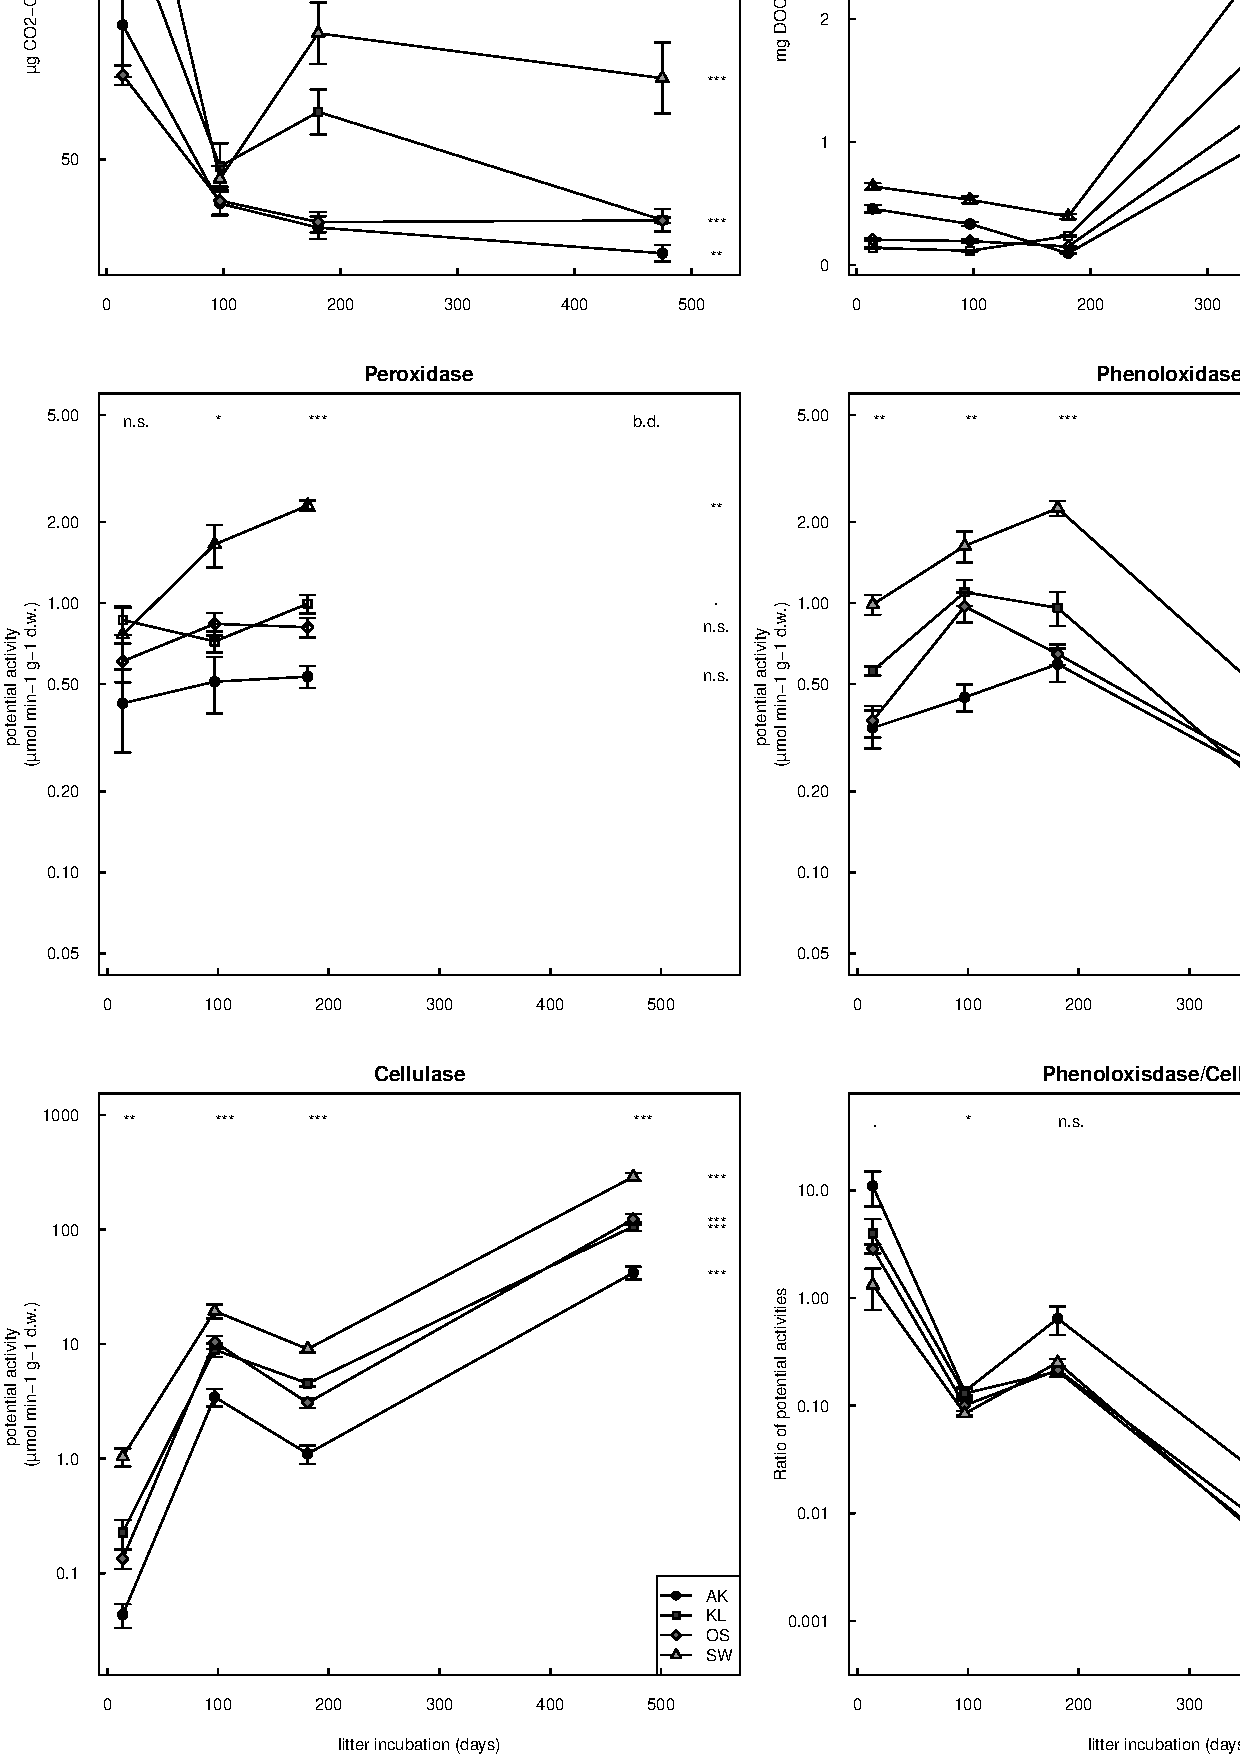
\includegraphics{ligpaper-enz}
\end{center}
%\caption{
%{\bf Respiration rates, concentration of soluble organic C and potential extracellular enzyme activities} in decomposing beech leaf litter from a mesocosm experiment. Beech litter was collected in: triangles, Schottenwald (SW); diamonds, Ossiach (OS); squares, Klaus-nleopoldsdorf (KL); circles, Achenkirch, AK. Error bars indicate standard errors (n=5). Significant differences between litter types are presented by asterisks above the symbols, significant differences between time points by asterisks to the right of the curves. *, P\textless 0.05, **, P\textless 0.01, ***, P\textless 0.001, b.d. - below detection limit.}
%\label{fig:enz}
\end{figure}

\begin{figure}[!ht]
\begin{center}
%\setkeys{Gin}{width=4in}
\setkeys{Gin}{width=\textwidth}
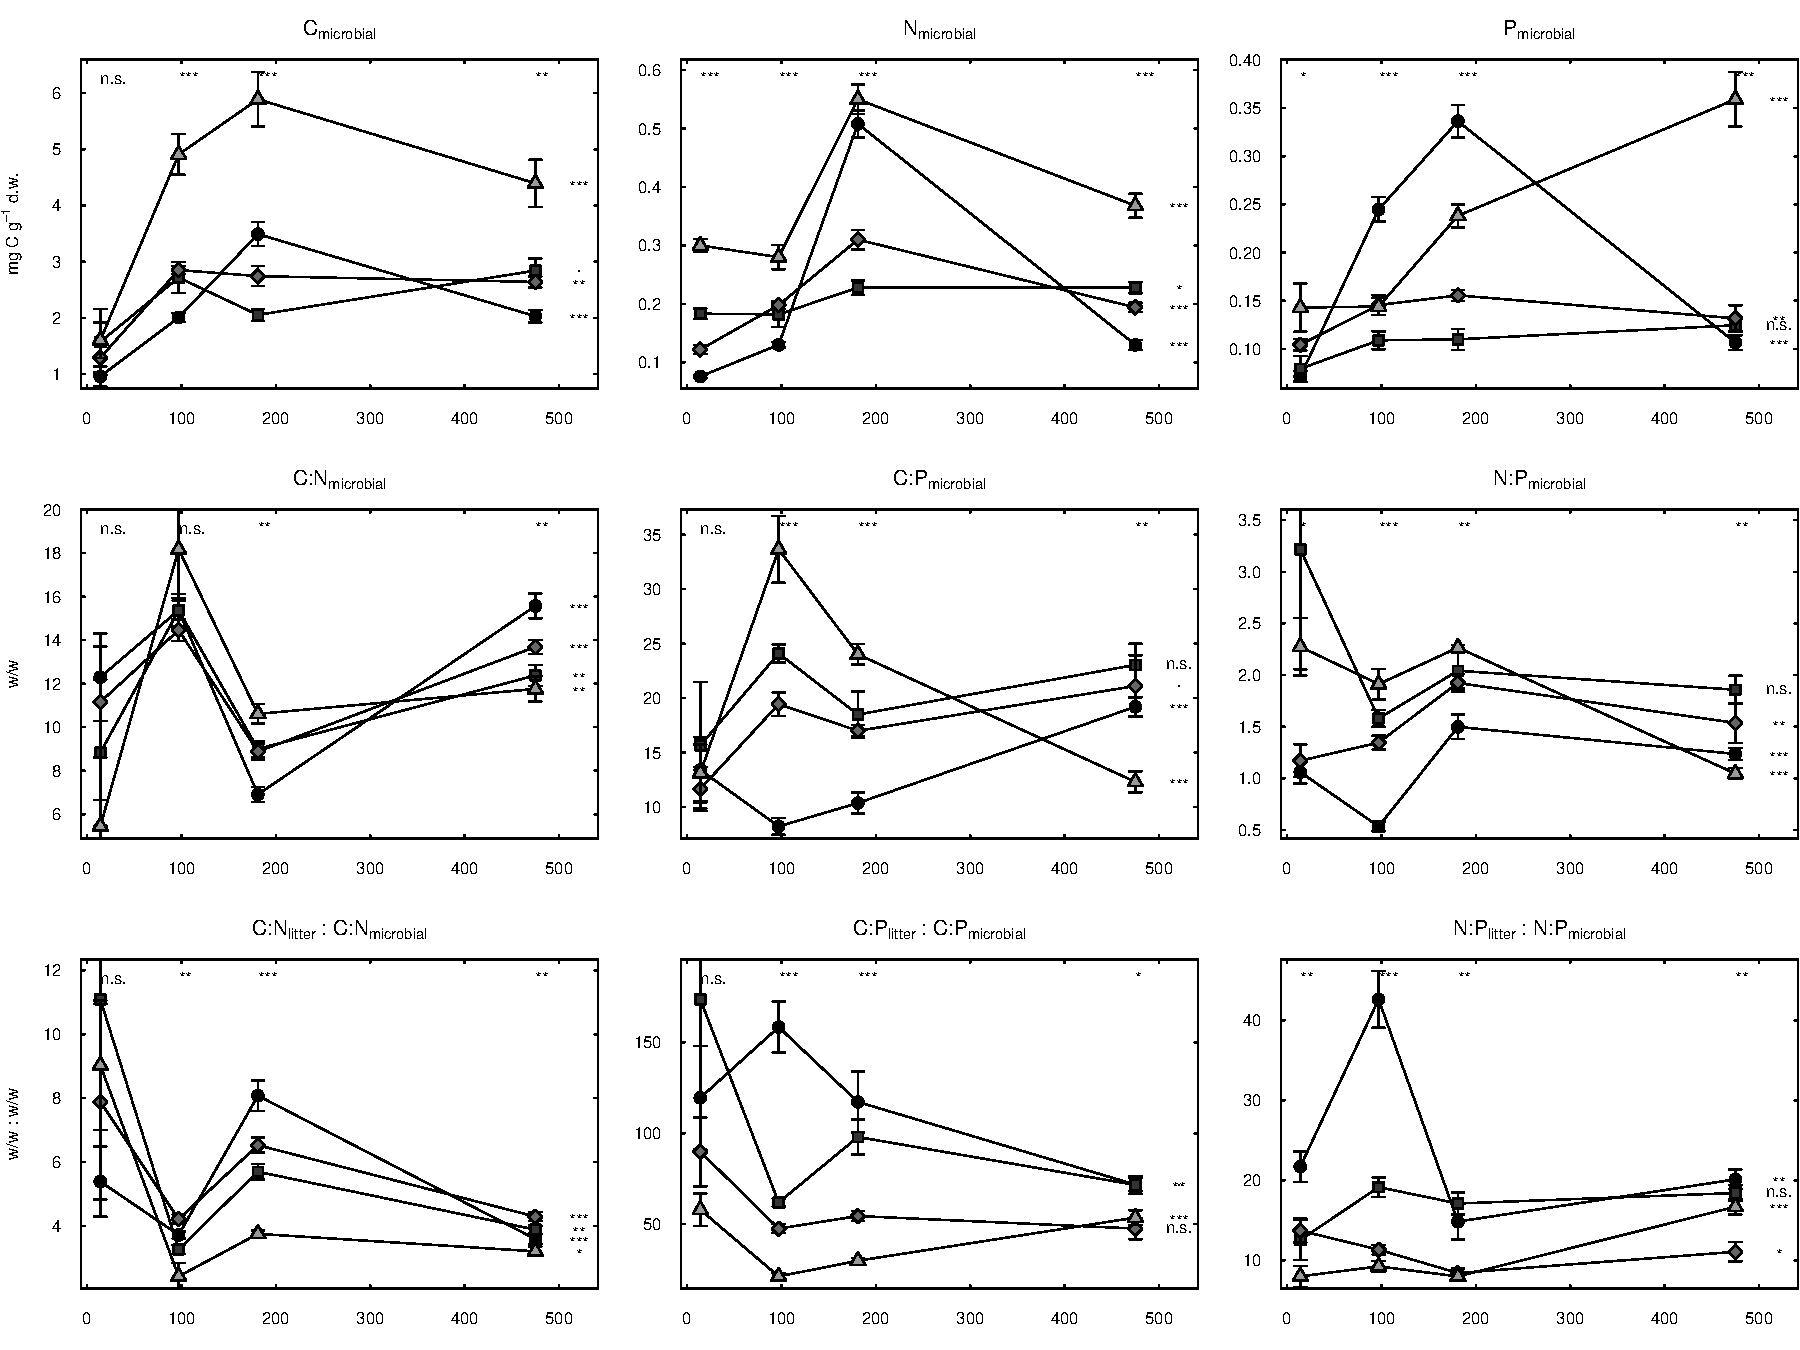
\includegraphics{ligpaper-mb}
\end{center}
%\caption{
%{\bf Microbial biomass C, N and P, microbial C:N:P stoichiometry and resource:consumer stoichiometric imbalance in these elements} in decomposing beech leaf litter from a mesocosm experiment. Beech litter was collected in: triangles, Schottenwald (SW); diamonds, Ossiach (OS); squares, Klausenleopoldsdorf (KL); circles, Achenkirch, AK. Error bars indicate standard errors (n=5). Significant differences between litter types are presented by asterisks above the symbols, significant differences between time points by asterisks to the right of the curves. *, P\textless 0.05, **, P\textless 0.01, ***, P\textless 0.001.}
%\label{fig:mb}
\end{figure}

\begin{figure}[!h]
\begin{center}
%\setkeys{Gin}{width=4in}
%\setkeys{Gin}{width=\textwidth}
\includegraphics{ligpaper-figphos}
\end{center}
%\caption{
%{\bf Mobilization of litter P} (A) Insoluble litter P is mobilized into recycled P pools (dissolved and microbial biomass P) in lignin degrading litter (AK and KL), while the increase in biomass P on non lignin-degrading litter (OS and SW) origininates from soluble P. (B) correlation between mobilization of P and lignin accumulation, 0-6 months incubation. Beech litter was collected in: triangles, Schottenwald (SW); diamonds, Ossiach (OS); squares, Klausenleopoldsdorf (KL); circles, Achenkirch, AK. Error bars indicate standard errors (n=5).}
%\label{fig:phos}
\end{figure}


\newpage
\begin{figure*}[h!]
\vspace*{2mm}
\begin{center}
\setkeys{Gin}{width=\textwidth}
\includegraphics{ligpaper-metaprot2}
\end{center}
%\caption{
%{\bf Protein abundance of fungal and bacterial taxa.} Litter was collected in Achenkirch (AK);, Klausenleopoldsdorf (KL); Ossiach (OS); Schottenwald (SW). Samples were analyzed after sterilization, re-innoculation and incubation for 14, 97, 181, or 475 days.}
%\label{fig:metaprot_barplot}
\end{figure*}


\begin{figure}[!ht]
\begin{center}
\setkeys{Gin}{width=0.7\textwidth}
%\inputgraphics[width=4in]{figure_name.2.eps}
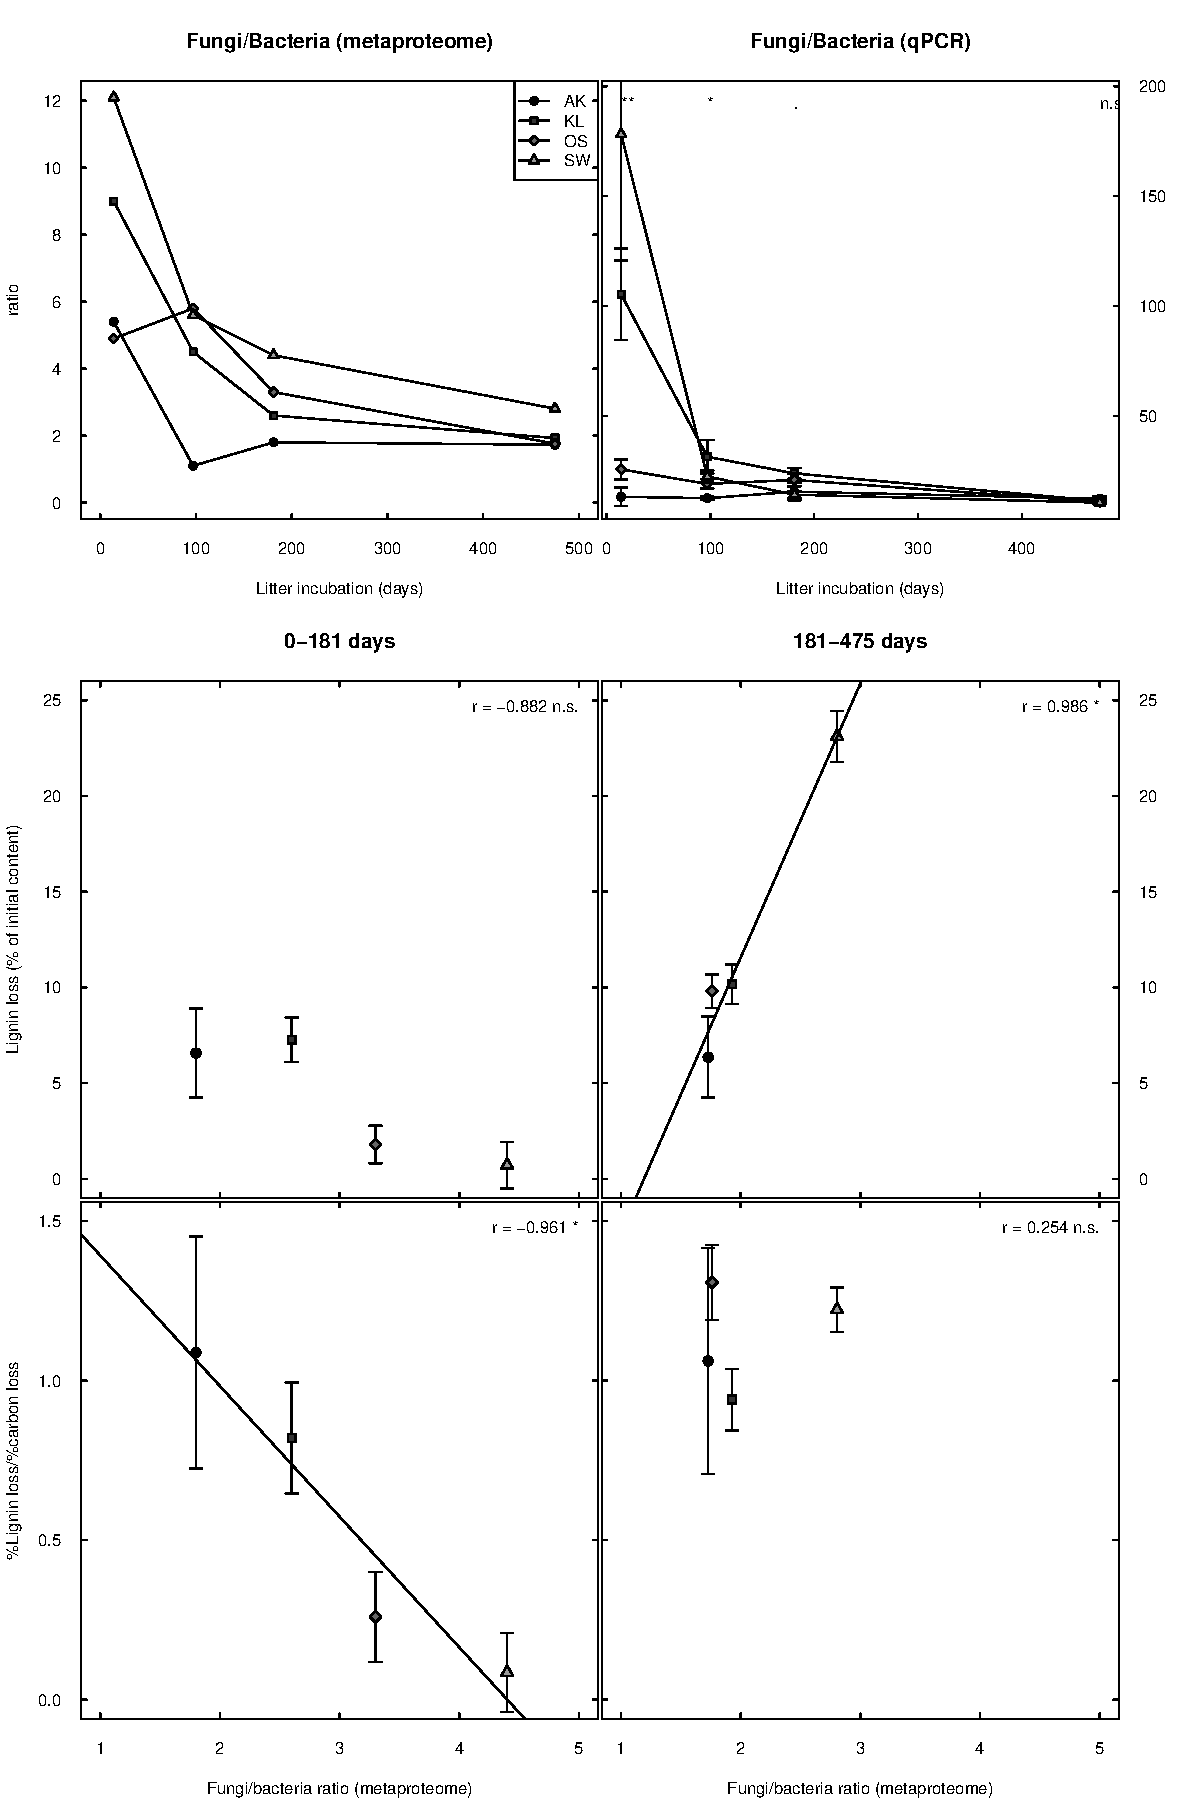
\includegraphics{ligpaper-f2bnew}
\end{center}
%\caption{
%{\bf Fungi:Bacteria (F:B) ratios and their correlations with LCI change:} A: F:B protein abundance (left) and DNA (right) ratio. B: Correlations between F:B preotein abundance ratios and lignin loss (top), carbohydrate loss (mid) and lignin loss : carbon loss (bottom) for 0-6 months (left) and 6-15 months (right, errorbars indicate standard errors, n=4-5).  Beech litter was collected in: triangles, Schottenwald (SW); diamonds, Ossiach (OS); squares, Klausenleopoldsdorf (KL); circles, Achenkirch, AK. Error bars indicate standard errors (n=5). Significant differences between litter types are presented by asterisks above the symbols, significant differences between time points by asterisks to the right of the curves. *, P\textless 0.05, **, P\textless 0.01, ***, P\textless 0.001.}
%\label{fig:f2b}
\end{figure}

\newpage
\begin{figure}[!ht]
\begin{center}
%\setkeys{Gin}{width=4in}
\setkeys{Gin}{width=\textwidth}
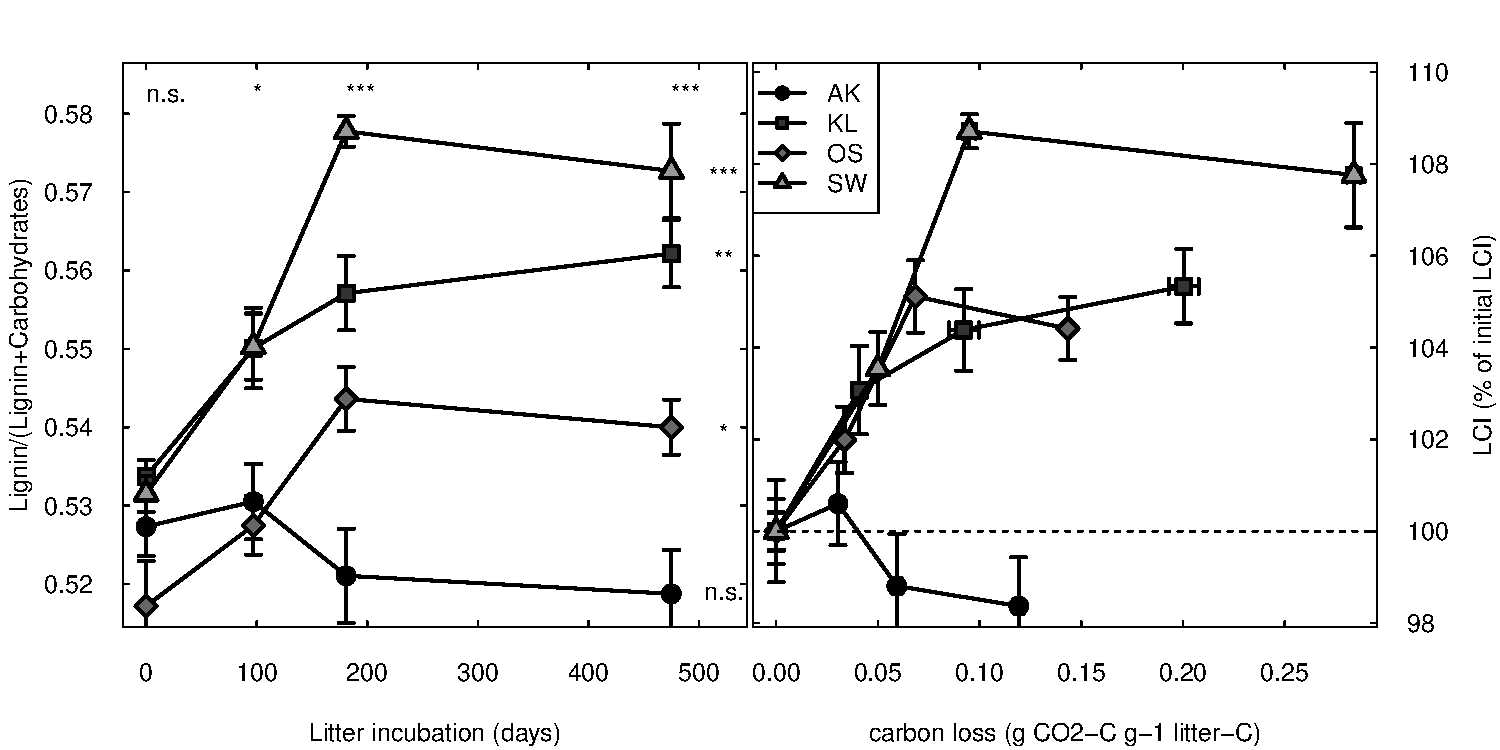
\includegraphics{ligpaper-lci}
\end{center}
%\caption{
%{\bf Develoment of lignin to carbohydrate index (lignin : (lignin+carbohydrates), LCI)} during time of beech litter decomposition (left) or plotted against cumulative C loss (right). Errorbars indicate standard errors (n=4-5). The dashed line indicates a constant ratio between lignin and carbohydrates (i.e. no preferential decomposition of carbohydrates. Beech litter was collected in: triangles, Schottenwald (SW); diamonds, Ossiach (OS); squares, Klausenleopoldsdorf (KL); circles, Achenkirch, AK. Error bars indicate standard errors (n=5). Significant differences between litter types are presented by asterisks above the symbols, significant differences between time points by asterisks to the right of the curves. *, P\textless 0.05, **, P\textless 0.01, ***, P\textless 0.001.}
%\label{fig:lci}
\end{figure}


\newpage
\begin{figure*}[h!]
\vspace*{2mm}
\begin{center}
\setkeys{Gin}{width=\textwidth}
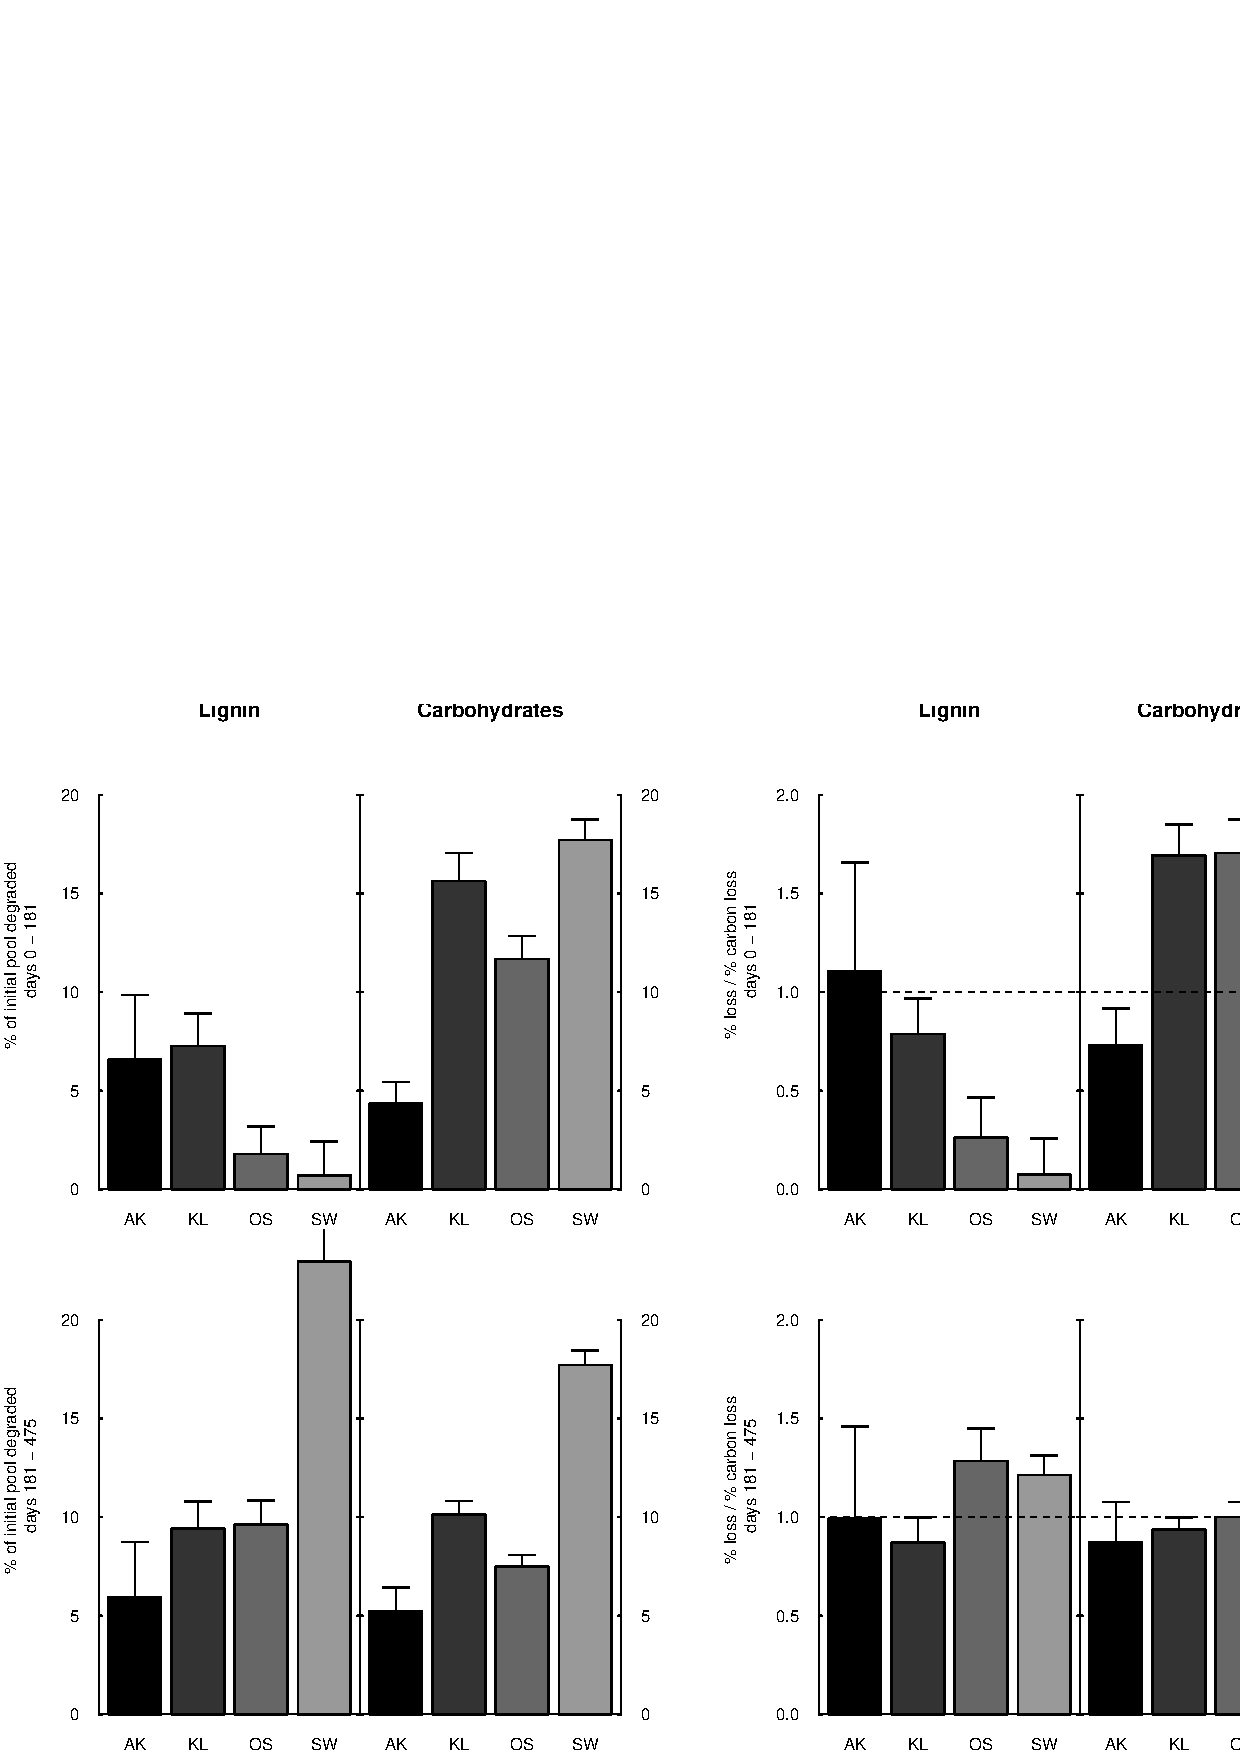
\includegraphics{ligpaper-degrdiff}
\end{center}
%\caption{
%{\bf Carbon loss corrected amounts of lignin and carbohydrates} degraded in beech litter collected in Achenkirch (AK), Klausenleopoldsdorf (KL), Ossiach (OS) and Schottenwald (SW). Carbon loss was calculated based on accumulated respiration for each mesocosm. Error bars indicate standard errors (n=4-5). The dashed line marks no discrimation during decomposition between lignin, carbohydrates and bulk carbon}
%\label{fig:degr}
\end{figure*}

\newpage
\begin{figure*}[h!]
\vspace*{2mm}
\begin{center}
\setkeys{Gin}{width=\textwidth}
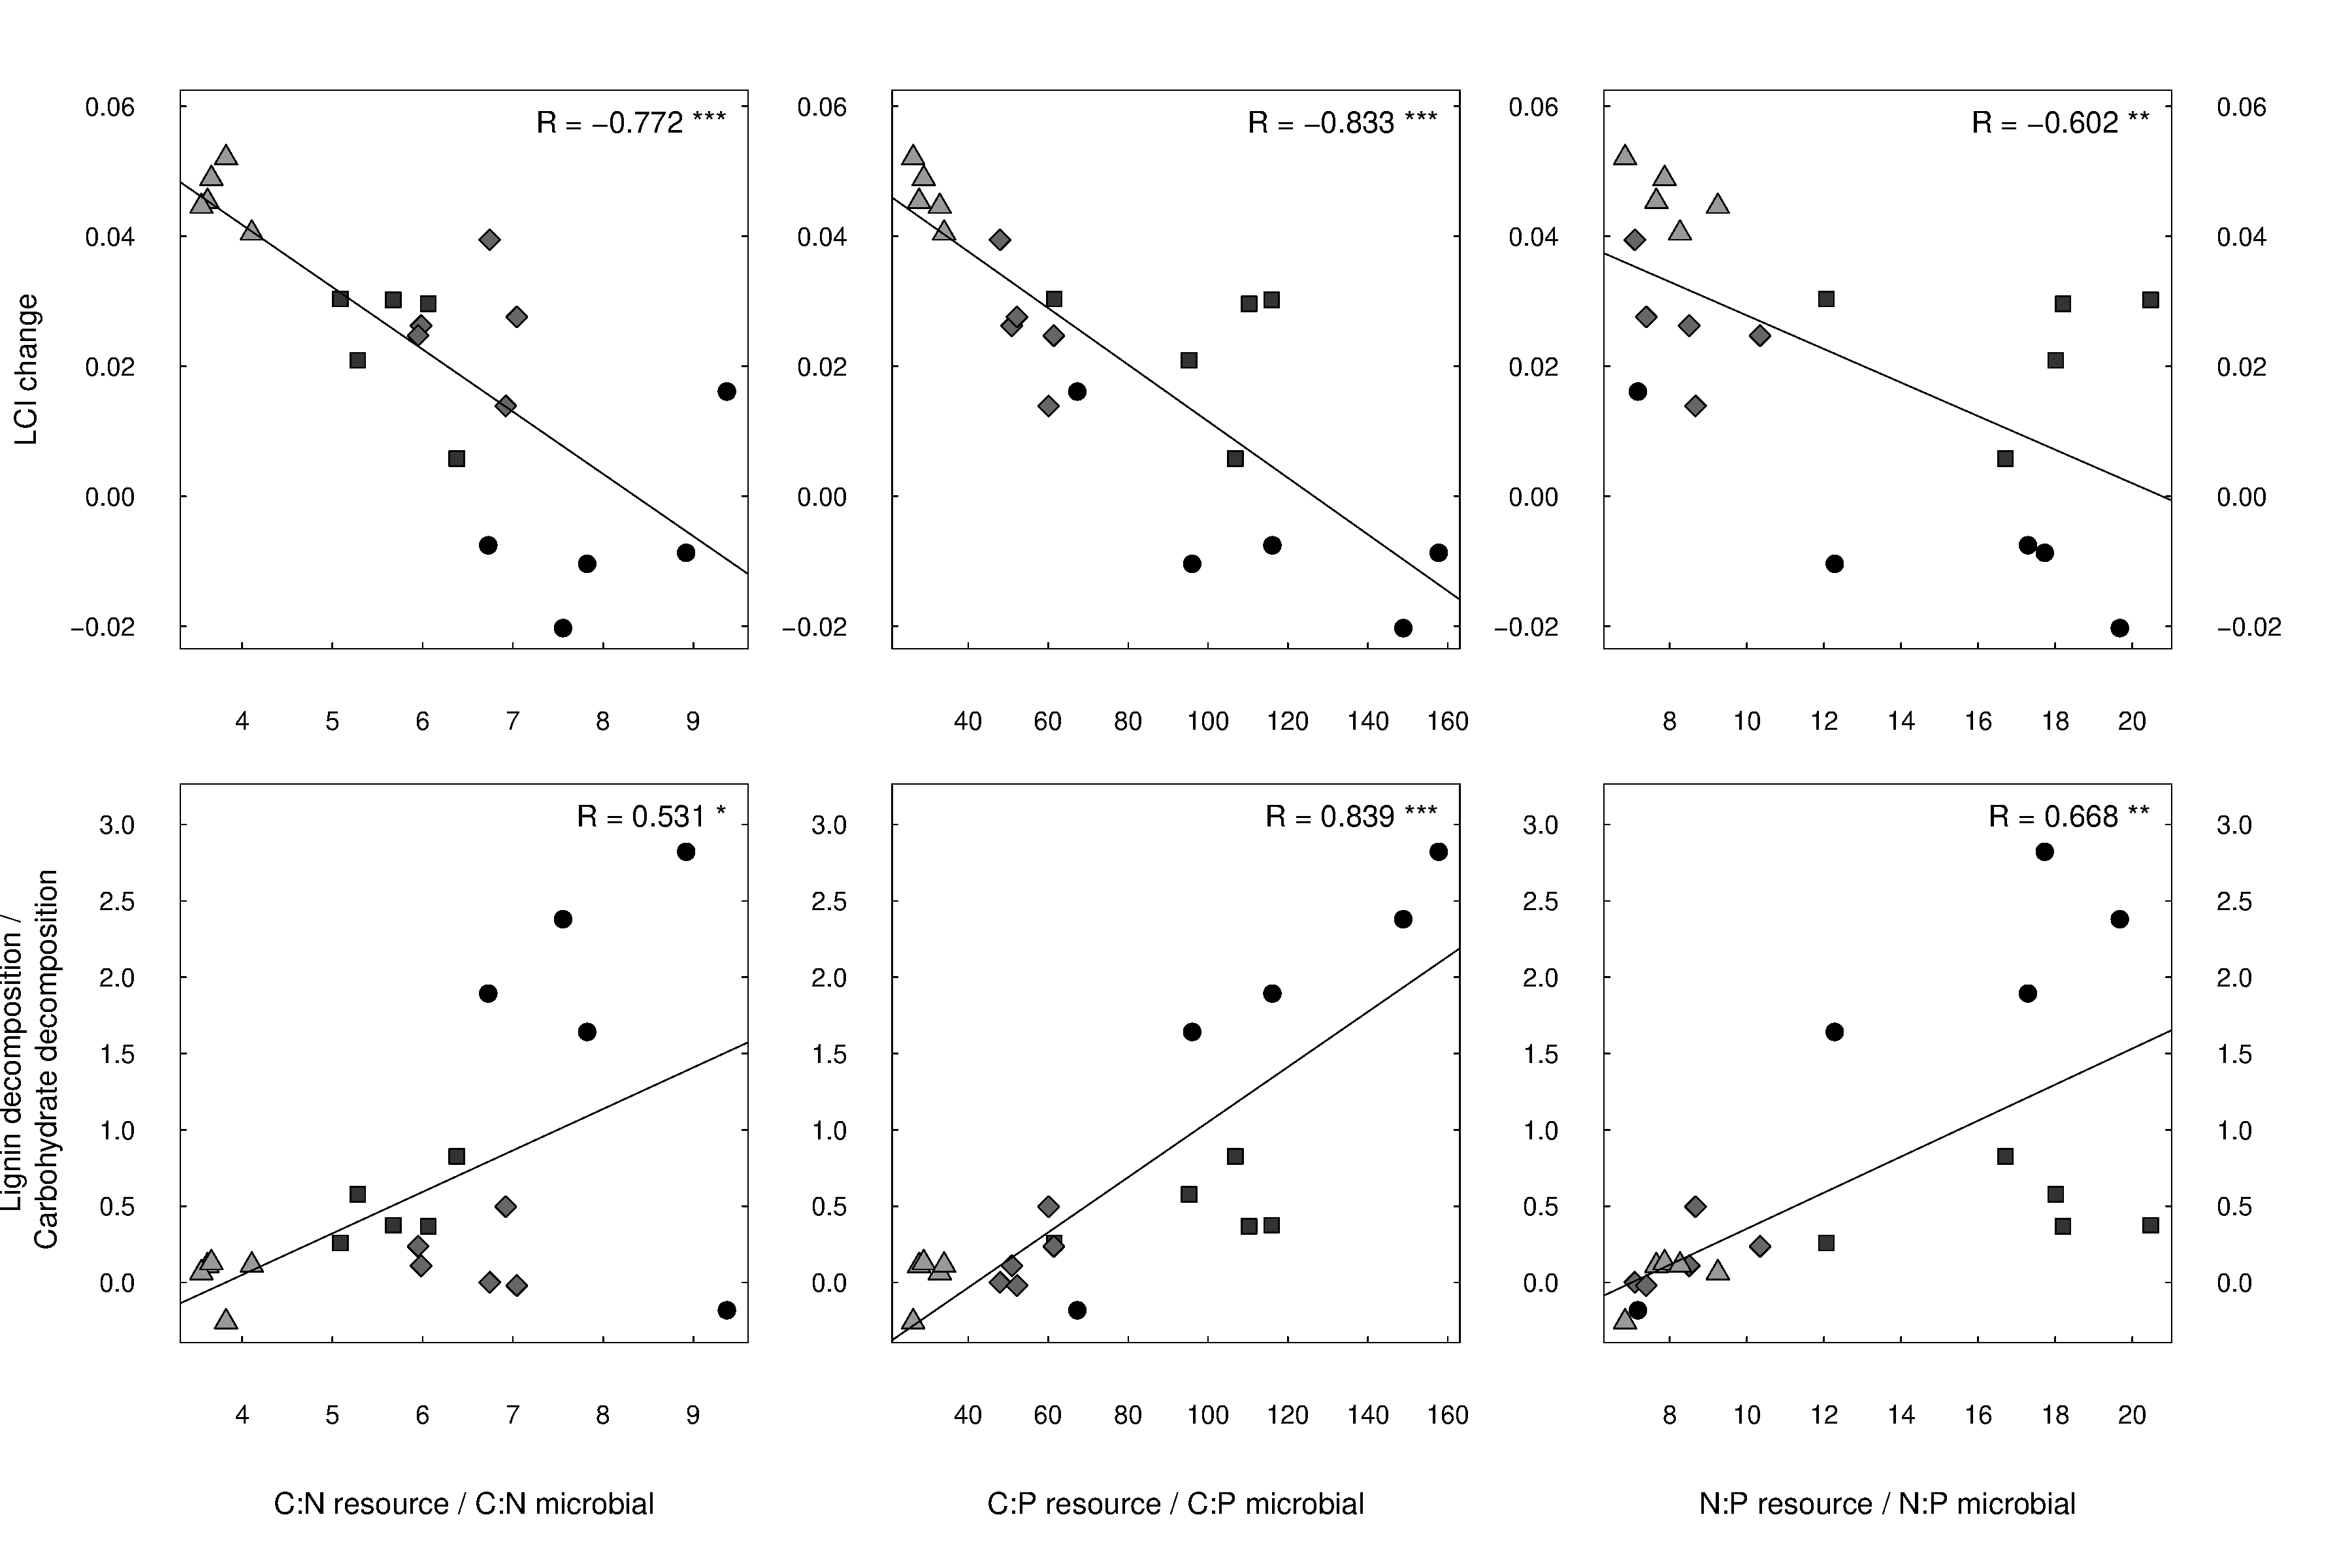
\includegraphics{ligpaper-graphcorr}
\end{center}
%\caption{
%{\bf Correlation between the LCI change or the ratio of lignin : carbohydrate decomposition ratio during the first 6 months of litter decomposition correlate to litter : microbe stoichiometric imbalances.} and change and Correlations between lignin accumulation during the first 6 month of litter incubation and stoichiometric resource:consumer imbalances. LCI is calculates as of lignin/(lignin+Carbohydrates).  Beech litter was collected in: triangles, Schottenwald (SW); diamonds, Ossiach (OS); squares, Klausenleopoldsdorf (KL); circles, Achenkirch, AK. *, P\textless 0.05, **, P\textless 0.01, ***, P\textless 0.001.}
%\label{fig:cor1}
\end{figure*}




\newpage
\begin{figure*}[h!]
\vspace*{2mm}
\begin{center}
\setkeys{Gin}{width=\textwidth}
\includegraphics{ligpaper-metaprot_pca}
\end{center}
%\caption{
%{\bf Microbial commuity composition.} The first two components of a correspondance analysis (CA) of protein abundances found. Rectangles indicate samples of identical incubation time. Peptides were aggregated at class level (fungi and proteobacteria) or phylum level (other bacterial phyla): Dothideomycetes (Doth); Eurotiomycetes (Euro); Leotiomycetes (Leot); Saccharomycetes (Sacc); Sordariomycetes (Sord); Agaricomycetes (Agar); Tremellomycetes (Trem); Ustilaginomycetes (Usti); Thermotogae (Ther); Bacteroidetes (Bact); Actinobacteria (Acti); Cyanobacteria (Cyan); Firmicutes (Firm); Fusobacteria (Fuso); Verrucomicrobia (Verr); Dictyoglomi (Dict); Alphaproteobacteria (Alph); Betaproteobacteria (Beta); Gammaproteobacteria (Gamm); Deltaproteobacteria (Delt); Epsilonproteobacteria (Epsi). Taxa factor loadings were printed x2 for better readability. Correlations between CA 1, CA 2, and litter chemistry, microbial stoichiometry, and protein abundance of microbial taxa are stated in supplemental table \ref{catab}. 
%Arrows represent vectorial fittings of these variables calculated independently from the CA, plotted only if p\textless 0.05: Litter C content (C lit); C:X\textsubscript{Microbial}/C:X\textsubscript{Litter} (C:P imb, C:N imb).}
%\label{fig:metaprotpca}
\end{figure*}

\newpage
\section*{Tables}

\begin{landscape}
% latex table generated in R 2.12.1 by xtable 1.5-6 package
% Sat Nov  5 23:56:54 2011
\begin{table}[h!]
%\begin{center}
\caption{Element concentrations, elemental stoichiometry and cellulose and lignin concentrations in beech litter measured after 14 days incubation. Standard errors are given in brackets (n=5). C extr represents for soluble organic carbon. Beech litter was collected in AK, Achenkirch, KL, Klausenleopoldsdorf, OS, Ossiach, and SW, Schottenwald.}
\label{initstoech}

{\small
\begin{tabular}{lrlrlrlrlrlr}
  \hline
 & AK & (SE) & KL & (SE) & OS & (SE) & SW & (SE) & p value \\ 
  \hline
C (\% d.w.) & 50.86 & (0.39) & 49.41 & (0.53) & 48.15 & (0.39) & 48.90 & (0.34) & 0.002 \\ 
  C extr (mg g-1) & 0.46 & (0.03) & 0.14 & (0.01) & 0.21 & (0.01) & 0.64 & (0.03) & $<$0.001 \\ 
  N (\% d.w.) & 0.878 &  (0.012) & 0.938 &  (0.012) & 0.806 &  (0.013) & 1.172 &  (0.016) & $<$0.001 \\ 
  P (\% d.w.) & 0.040 & (0.000) & 0.030 & (0.000) & 0.052 & (0.002) & 0.070 & (0.000) & $<$0.001 \\ 
  C:N (w/w) & 57.86 &  (0.57) & 52.60 &  (0.49) & 59.97 &  (0.72) & 41.78 &  (0.76) & $<$0.001 \\ 
  C:P (w/w) & 1282 & (21) & 1548 & (25) & 905 & (15) & 699 & (9) & $<$0.001 \\ 
  N:P (w/w) & 22.17 & (0.47) & 29.45 & (0.60) & 15.10 & (0.29) & 16.75 & (0.39) & $<$0.001 \\ 
  K (mg g-1) & 0.26 & (0.00) & 0.54 & (0.00) & 0.21 & (0.00) & 0.55 & (0.00) & $<$0.001 \\ 
  Ca (mg g-1) & 1.33 & (0.01) & 1.26 & (0.01) & 1.63 & (0.01) & 1.23 & (0.01) & $<$0.001 \\ 
  Mg (mg g-1) & 0.27 &  (0.00) & 0.14 &  (0.00) & 0.20 &  (0.00) & 0.15 &  (0.00) & $<$0.001 \\ 
  Fe (ppm) & 210 & (2) & 208 & (4) & 453 & (12) & 192 & (4) & $<$0.001 \\ 
  Mn (ppm) & 172 &  (2) & 1430 &  (10) & 776 &  (9) & 2137 &  (51) & $<$0.001 \\ 
  Zn (ppm) & 30.8 & (0.4) & 33.0 & (0.3) & 36.0 & (1.0) & 42.4 & (0.7) & $<$0.001 \\ 
  Lignin & 28.9 & (28.9) & 29.9 & (29.9) & 31.2 & (31.2) & 30.5 & (30.5) & $<$0.001 \\ 
  Carbohydrates & 25.9 & (25.9) & 26.1 & (26.1) & 29.2 & (29.2) & 26.9 & (26.9) & $<$0.001 \\ 
   \hline
\end{tabular}
}
%\end{center}
\end{table}
\end{landscape}




%\section*{Supporting Information}



%\begin{table}[h!]
\begin{center}
\caption{Lignin derived and other phenolic pyrolysis products}
\label{tab:phprod}

{\small
\begin{tabular}{lcccccc}
  \hline
Name & RT & MW & integrated framents & Origin & Class \\ 
  \hline
Guaiacol & 18.87 & 124 & 109+124 &Lignin&Guaiacyl\\ 
Methylguaiacol & 20.32 & 138 & 123+138 &Lignin&Guaiacyl\\ 
Ethylguaiacol & 21.40 & 152 & 137+152 &Lignin&Guaiacyl\\ 
Propenylguaiacol & 23.29 & 164 & 149+164 &Lignin&Guaiacyl\\ 
Vinylguaiacol & 23.69 & 150 & 135+150 &Lignin&Guaiacyl\\ 
Propenylguaiacol & 24.48 & 164 & 149+164 &Lignin&Guaiacyl\\ 
Syringol & 24.58 & 154 & 139+154 &Lignin&Syringyl\\ 
Propenylguaiacol & 25.66 & 164 & 149+164 &Lignin&Guaiacyl\\ 
Methylsyringol & 25.67 & 168 & 153+168 &Lignin&Syringyl\\ 
Ethylsysringol & 26.39 & 182 & 167+182 &Lignin&Syringyl\\ 
Propenylsyringol & 27.97 & 194 & 179+194 &Lignin&Syringyl\\ 
Vinylsyringol & 28.37 & 180 & 165+180 &Lignin&Syringyl\\ 
Guaiacolaldehyde & 28.40 & 152 & 109+152 &Lignin&Guaiacyl\\ 
Propylguaiacol & 28.72 & 166 & 137+166 &Lignin&Guaiacyl\\ 
Oxo-hydroxy-etylguaiacol & 28.77 & 182 & 182 &Lignin&Guaiacyl\\ 
Propenylsyringol & 28.91 & 194 & 179+194 &Lignin&Syringyl\\ 
Oxo-ethylguaiacol & 29.20 & 166 & 151+166 &Lignin&Guaiacyl\\ 
Oxo-propylguaiacol & 29.36 & 180 & 137+180 &Lignin&Guaiacyl\\ 
Propenylsyringol & 30.16 & 194 & 194+179 &Lignin&Syringyl\\ 
Syringolaldehyde & 32.68 & 182 & 139+182 &Lignin&Syringyl\\ 
Oxo-hydroxy-ethylsyringol & 32.80 & 212 & 212 &Lignin&Syringyl\\ 
Guaiacolacetic acid & 32.88 & 182 & 137+182 &Lignin&Guaiacyl\\ 
Propylsyringol & 33.15 & 196 & 181+196 &Lignin&Syringyl\\ 
Oxo-propylsyringol & 33.32 & 210 & 167+210 &Lignin&Syringyl\\ 
Oxopropenylguaiacol & 35.30 & 178 & 135+178 &Lignin&Guaiacyl\\ 
Hydroxypropenylguaiacol & 37.10 & 180 & 137+180 &Lignin&Guaiacyl\\ 
Syringolacetic acid & 38.78 & 212 & 212 &Lignin&Syringyl\\ 
Oxo-propenylsyringol & 43.06 & 208 & 165+208 &Lignin&Syringyl\\ 
Phenol & 21.02 & 94 & 65+66+94 &Phenolic&\\ 
4-Methylphenol & 22.11 & 108 & 107+108 &Phenolic&\\ 
3-Methylphenol & 22.22 & 108 & 107+108 &Phenolic&\\ 
Ethylphenol & 23.38 & 122 & 107+122 &Phenolic&\\ 
Propenylphenol & 26.93 & 134 & 133+134 &Phenolic&\\ 
Propenylphenol & 27.76 & 134 & 133+134 &Phenolic&\\ 
Propylphenol & 31.11 & 136 & 151+166 &Phenolic&\\ 
Butylphenol & 31.86 & 150 & 107+150 &Phenolic&\\ 
4-Hydroxybenzaldehyde & 32.70 & 122 & 121+122 &Phenolic&\\ 
Hydroquinone & 33.40 & 110 & 81+110 &Phenolic&\\ 
   \hline
\end{tabular}
}
\end{center}
\end{table}
\newpage

% latex table generated in R 2.12.1 by xtable 1.6-0 package
% Tue Nov  8 06:46:38 2011
\begin{table}[h!]
\begin{center}
\caption{Carbohydrate derived pyrolysis products}
\label{tab:chprod}
{\small
\begin{tabular}{lcccccc}
  \hline
Name & RT & MW & integrated framents & Origin & Class \\ 
  \hline
Acetaldehyde & 2.06 & 44 & 29+44 &Carbohydrates&  \\ 
Furan & 2.35 & 68 & 39+68 &Carbohydrates&Furan\\ 
Methylfuran & 2.74 & 82 & 81+82 &Carbohydrates&Furan\\ 
Methylfuran & 2.91 & 82 & 81+82 &Carbohydrates&Furan\\ 
Dimethylfuran & 3.43 & 96 & 95+96 &Carbohydrates&Furan\\ 
Dimethylfuran & 3.66 & 96 & 95+96 &Carbohydrates&Furan\\ 
Vinylfuran & 5.01 & 94 & 65+94 &Carbohydrates&Furan\\ 
Unknown furan & 6.36 & 108 & 107+108 &Carbohydrates&Furan\\ 
Cyclopentanone & 6.99 & 105 & 84+105 &Carbohydrates&Cyclopentenone\\ 
Methylfuran & 7.62 & 82 & 53+82+83 &Carbohydrates&Furan\\ 
2-Oxopropanoic acid, methylester & 7.92 & 102 & 43+102 &Carbohydrates& \\ 
1-Hydroxypropanone & 9.24 & 74 & 43 &Carbohydrates& \\ 
2-Cyclopenten-1-one & 10.26 & 82 & 53+54+52 &Carbohydrates&Cyclopentenone\\ 
2-Methyl-2-cyclopenten-1-one & 10.51 & 96 & 53+96 &Carbohydrates&Cyclopentenone\\ 
1-Hydroxy-2-propanone & 10.69 & 88 & 57+88 &Carbohydrates&Cyclopentenone\\ 
Unknown & 11.38 & unk & 65+66+94 &Carbohydrates& \\ 
3-Furaldehyd & 11.57 & 96 & 95+96 &Carbohydrates&Furan\\ 
2(5H)Furanon & 11.69 & 98 & 55+98 &Carbohydrates&Furan\\ 
Propanoic acid, methylester & 12.10 & 102 & 43+102 &Carbohydrates& \\ 
2-Furaldehyd & 12.22 & 96 & 95+96 &Carbohydrates&Furan\\ 
Acetylfuran & 12.99 & 110 & 95+110 &Carbohydrates&Cyclopentenone\\ 
3-Methyl-cyclopentanone & 13.31 & 96 & 67+96 &Carbohydrates&Cyclopentenone\\ 
Dimethylcyclopentenone & 13.69 & 110 & 67+95+110 &Carbohydrates&Cyclopentenone\\ 
5-Methyl-2-furancarboxaldehyde & 14.23 & 110 & 109+110 &Carbohydrates&Furan\\ 
2-Cyclopenten-1,4-dione & 14.44 & 96 & 54+68+96 &Carbohydrates&Cyclopentenone\\ 
Butyrolactone & 15.22 & 86 & 56+86 &Carbohydrates& \\ 
Unknown & 15.56 &  &  &Carbohydrates&  \\ 
Furanmethanol & 15.61 & 98 & 98 &Carbohydrates&Cyclopentenone\\ 
5-Methyl-2(5H)-furanone & 16.06 & 98 & 55+98 &Carbohydrates&Furan\\ 
Unknown & 16.17 & unk & 110 &Carbohydrates&  \\ 
1,2-Cylopentandione & 17.51 & 98 & 55+98 &Carbohydrates&Cyclopentenone\\ 
Unknown & 17.67 & unk & 42+70 &Carbohydrates&  \\ 
2-Hydroxy-3-methyl-2-cyclopenten-1-one & 18.14 & 98 & 98 &Carbohydrates&Cyclopentenone\\ 
3-Methy-l1,2-cyclopentanedione & 18.42 & 112 & 69+112 &Carbohydrates&Cyclopentenone\\ 
Unknown & 19.06 && 58+86+114 &Carbohydrates&\\ 
Unknown & 19.35 && 98+126 &Carbohydrates&\\ 
Unknown & 21.77 && 116 &Carbohydrates&\\ 
Unknown & 22.33 && 44 &Carbohydrates&\\ 
Unknown & 26.18 && 57+69 &Carbohydrates&\\ 
5-Hydroxymethylfuran-1-carboxaldehyde & 27.51 & 126 & 97+126 &Carbohydrates&Furan\\ 
Unknown & 31.67 && 73+135 &Carbohydrates&\\ 
Laevoglucosan & 40.44 & 172 & 60+73 &Carbohydrates& \\ 
   \hline
\end{tabular}
}
\end{center}
\end{table}


\newpage
% latex table generated in R 2.12.1 by xtable 1.6-0 package
% Tue Nov  8 06:46:38 2011
\begin{table}[h!]
\begin{center}
\caption{Other pyrolysis products}
\label{tab:nprod}
{\small
\begin{tabular}{lcccccc}
  \hline
Name & RT & MW & integrated framents & Origin & Class \\ 
  \hline
25:0 Alkan & 27.74 & 352 & 57+71 &aliphatic& Alkan \\ 
25:1 Alken & 28.34 & 350 & 57+69 &aliphatic& Alken \\ 
27:0 Alkan & 30.04 & 380 & 57+67 &aliphatic& Alkan \\ 
27:1 Alken & 30.63 & 378 & 57+65 &aliphatic& Alken \\ 
29:0 Alkan & 32.20 & 408 & 57+63 &aliphatic& Alkan \\ 
29:1 Alken & 32.82 & 406 & 57+61 &aliphatic& Alken \\ 
Myristic acid (14:0) & 2.35 & 68 & 39+68 & Lipid & Fatty Acid \\ 
Palmitic acid (16:0) & 2.74 & 82 & 81+82 & Lipid & Fatty Acid \\ 
Stearuc acid (18:0) & 2.91 & 82 & 81+82 & Lipid & Fatty Acid \\ 
N-methyl-pyrrol & 6.15 & 81 & 80+81 &Protein& Pyrrol \\ 
Pyridine & 6.90 & 95 & 52+79+95 &Protein& Pyridine \\ 
Methylpyridine & 7.50 & 93 & 66+92+93 &Protein& Pyridine \\ 
Methylpyridine & 7.54 & 93 & 66+92+93 &Protein& Pyridine \\ 
methylpyridine & 9.02 & 93 & 66+93 &Protein& Pyridine \\ 
Pyrrol & 13.11 & 67 & 39+41+67 &Protein& Pyrrol \\ 
Methylpyrrol & 13.81 & 81 & 80+81 &Protein& Pyrrol \\ 
Methylpyrrol & 14.10 & 81 & 80+81 &Protein& Pyrrol \\ 
3-Hydroxypyridine & 26.52 & 95 & 67+95 &Protein& Pyridine \\ 
Indole & 26.85 & 117 & 89+117 &Protein& Indole \\ 
Methylindole & 27.42 & 131 & 130+131 &Protein& Indole \\ 
Toluene & 4.54 & 92 & 91+92 &&Aromatic\\ 
Xylene & 5.94 & 106 & 91+105+106 &&Aromatic\\ 
Xylene & 6.09 & 106 & 91+105+106 &&Aromatic\\ 
Xylene & 6.20 & 106 & 91+105+106 &&Aromatic\\ 
Xylene & 6.99 & 105? & 84+105? &&Aromatic\\ 
Methoxytoluene & 11.78 & 122 & 121+122 &&Aromatic\\ 
Indene & 12.64 & 116 & 115+116 &&Aromatic\\ 
Benzaldehyde & 13.35 & 106 & 77+106 &&Aromatic\\ 
Dihydrobenzofuran & 26.19 & 120 & 91+119+120 &  & Aromatic \\ 
Limonene & 7.22 & 136 & 93 && Terpene \\ 
Phytol & 20.00 & 276 & 95+123 & Chlorophyll & Terpene \\ 
Unknown aliphatic & 22.82 && 58+71 && aliphatic \\ 
Aceton & 2.46 & 58 & 43 &  &  \\ 
2-Propenal & 2.60 & 56 & 55+56 &  &\\ 
Methanol & 2.88 & 32 & 29+31+32 &  &\\ 
3-Buten-2-one & 3.39 & 70 & 55+70 &  &\\ 
2,3-Butandione & 3.67 & 86 & 69+86 &&\\ 
3-Penten-2-one & 3.89 & 86 & 69+86 &&\\ 
2-Butanal & 4.56 & 70 & 69+70 &&\\ 
2,3-Pentadione & 4.77 & 100 & 57+100 &&\\ 
Hexanal & 5.16 & 82 & 56+72+82 &&\\ 
1-Penten-3-one & 11.28 & 84 & 55+84 &&\\ 
Hexan-2,4-dion & 23.92 & 114 & 56+84+114 &&  \\ 
unknown & 15.98 && 119+134 &&\\ 
Unknown & 20.85 && 81 &&\\ 
Unknown & 20.86 && 82+95 &&\\ 
Unknown & 22.43 && 98+128 &&\\ 
Unknown & 27.76 && 138 &&\\ 
   \hline
\end{tabular}
}
\end{center}
\end{table}



\begin{landscape}

% latex table generated in R 2.15.2 by xtable 1.7-1 package
% Mon Sep  2 17:28:20 2013
\begin{table}[h!]
\centering
\caption{Results of correlation analysis (R) between lignin and carbohydrate decomposition and other decomposition processes (mass loss, respiration), extracellular enzyme activities, litter chemistry, and litter and microbial biomass C:N:P stoichiometry. Significant (p\textless 0.05) correlations are presented in bold. Data taken from \cite{Mooshammer2011, Leitner2011}. Changes in litter chemistry (lignin and carbohydrate decomposition) were calculated between 0 and 181 days, other data were measured after 181 days. $\Delta _{L}$, $\Delta _{Ch}$ - differences in lignin/carbydrate contents (pyr-GC/MS), $\Delta _{LCI}$ - LCI (lignin : (lignin + carbohydrates)) difference (pyr-GC/MS), $L_{degr}$, $Ch_{degr}$ - \% of initial lignin/carbohydrate loss, $L/C_{degr}$, $Ch/C_{degr}$  - \% lignin/carbohydrates loss : \% carbon respired, $L:Ch_{degr}$ - lignin loss : carbohydrate loss, Per:Cell - Potetial peroxidase activity : potential cellulase activity, Phen:Cell - Potetial phenoloxidase activity : potential cellulase activity.} 
\label{corrtable}
{\small
\begin{tabular}{lrrrrrrrrrr}
  \hline
 & $\Delta _{L}$ & $\Delta _{Ch}$ & $\Delta _{LCIC}$ & $L_{degr}$ & $Ch_{degr}$ & $L:C_{degr}$ & $Ch:C_{degr}$ & $L:Ch_{degr}$ & Per:Cell & Phen:Cell \\ 
  \hline
Massloss & 0.291 & -0.15 & 0.245 & -0.328 & 0.106 & -0.201 & 0.125 & -0.081 & 0.048 & 0.0534 \\ 
  Actual respiration & \textbf{ 0.569 } & \textbf{ -0.453 } & \textbf{ 0.565 } & \textbf{ -0.543 } & 0.392 & \textbf{ -0.503 } & \textbf{ 0.453 } & \textbf{ -0.458 } & -0.294 & -0.346 \\ 
  Accumulated Respiration & -0.149 & -0.32 & 0.114 &  0.4 & \textbf{ 0.446 } & 0.208 & 0.258 & -0.0982 & -0.251 & -0.347 \\ 
  Cellulase activity & \textbf{ 0.657 } & \textbf{ -0.76 } & \textbf{ 0.803 } & -0.431 & \textbf{ 0.801 } & \textbf{ -0.497 } & \textbf{ 0.664 } & \textbf{ -0.589 } & -0.436 & \textbf{ -0.539 } \\ 
  Protease activity & 0.186 & -0.296 & 0.264 & -0.132 & 0.274 & -0.157 & 0.301 & -0.27 & -0.26 & -0.18 \\ 
  Phosphatase activity & 0.409 & \textbf{ -0.749 } & \textbf{ 0.663 } & -0.17 & \textbf{ 0.795 } & -0.312 & \textbf{ 0.677 } & \textbf{ -0.559 } & \textbf{ -0.49 } & \textbf{ -0.607 } \\ 
  Chitinase activity & \textbf{ 0.549 } & \textbf{ -0.813 } & \textbf{ 0.776 } & -0.302 & \textbf{ 0.851 } & -0.407 & \textbf{ 0.702 } & \textbf{ -0.556 } & -0.418 & \textbf{ -0.522 } \\ 
  Phenoloxidase activity & \textbf{ 0.632 } & \textbf{ -0.669 } & \textbf{ 0.737 } & -0.415 & \textbf{ 0.719 } & \textbf{ -0.449 } & \textbf{ 0.552 } & \textbf{ -0.484 } & -0.305 & -0.356 \\ 
  Peroxidase activity & \textbf{ 0.599 } & \textbf{ -0.588 } & \textbf{ 0.677 } & -0.412 & \textbf{ 0.639 } & -0.438 & \textbf{ 0.47 } & -0.435 & -0.173 & -0.302 \\ 
  N mineralization & \textbf{ 0.466 } & \textbf{ -0.664 } & \textbf{ 0.65 } & -0.167 & \textbf{ 0.739 } & -0.299 & \textbf{ 0.527 } & -0.387 & -0.282 & -0.367 \\ 
  Nitrification & \textbf{ 0.587 } & \textbf{ -0.707 } & \textbf{ 0.732 } & -0.38 & \textbf{ 0.74 } & -0.432 & \textbf{ 0.621 } & \textbf{ -0.499 } & -0.369 & -0.45 \\ 
  P mineralization & \textbf{ 0.665 } & \textbf{ -0.55 } & \textbf{ 0.684 } & \textbf{ -0.544 } & \textbf{ 0.596 } & \textbf{ -0.576 } & 0.414 & \textbf{ -0.478 } & -0.212 & -0.255 \\ 
  C litter & \textbf{ -0.545 } & \textbf{ 0.506 } & \textbf{ -0.578 } & \textbf{ 0.604 } & -0.368 & \textbf{ 0.643 } & \textbf{ -0.618 } & \textbf{ 0.698 } & \textbf{ 0.525 } & \textbf{ 0.581 } \\ 
  extractable C & 0.318 & -0.015 & 0.197 & -0.268 & 0.0745 & -0.166 & -0.118 & 0.0531 & 0.203 & 0.203 \\ 
  N litter & 0.354 & \textbf{ -0.517 } & \textbf{ 0.503 } & -0.14 & \textbf{ 0.587 } & -0.187 & 0.366 & -0.203 & -0.119 & -0.159 \\ 
  P litter & \textbf{ 0.692 } & -0.262 & \textbf{ 0.543 } & \textbf{ -0.756 } & 0.204 & \textbf{ -0.689 } & 0.232 & \textbf{ -0.501 } & -0.0902 & -0.173 \\ 
  C:N litter & -0.405 & \textbf{ 0.586 } & \textbf{ -0.57 } & 0.175 & \textbf{ -0.654 } & 0.234 & -0.44 & 0.273 & 0.195 & 0.242 \\ 
  C:P litter & \textbf{ -0.636 } & 0.174 & \textbf{ -0.453 } & \textbf{ 0.754 } & -0.0823 & \textbf{ 0.649 } & -0.176 & 0.418 & 0.049 & 0.0805 \\ 
  N:P litter & \textbf{ -0.512 } & -0.0287 & -0.264 & \textbf{ 0.714 } & 0.147 & \textbf{ 0.577 } & -0.0202 & 0.316 & -0.0316 & -0.0192 \\ 
  C:N mic & \textbf{ 0.664 } & \textbf{ -0.758 } & \textbf{ 0.799 } & -0.428 & \textbf{ 0.798 } & \textbf{ -0.514 } & \textbf{ 0.678 } & \textbf{ -0.609 } & \textbf{ -0.583 } & \textbf{ -0.595 } \\ 
  C:P mic & \textbf{ 0.691 } & \textbf{ -0.786 } & \textbf{ 0.833 } & \textbf{ -0.475 } & \textbf{ 0.813 } & \textbf{ -0.561 } & \textbf{ 0.725 } & \textbf{ -0.671 } & \textbf{ -0.564 } & \textbf{ -0.647 } \\ 
  N:P mic & \textbf{ 0.582 } & \textbf{ -0.729 } & \textbf{ 0.74 } & -0.416 & \textbf{ 0.728 } & \textbf{ -0.508 } & \textbf{ 0.715 } & \textbf{ -0.67 } & \textbf{ -0.545 } & \textbf{ -0.672 } \\ 
  C:N imbalance & \textbf{ -0.559 } & \textbf{ 0.81 } & \textbf{ -0.772 } & 0.287 & \textbf{ -0.86 } & 0.39 & \textbf{ -0.71 } & \textbf{ 0.531 } & \textbf{ 0.563 } & \textbf{ 0.56 } \\ 
  C:P imbalance & \textbf{ -0.816 } & \textbf{ 0.663 } & \textbf{ -0.833 } & \textbf{ 0.756 } & \textbf{ -0.61 } & \textbf{ 0.798 } & \textbf{ -0.668 } & \textbf{ 0.838 } & \textbf{ 0.576 } & \textbf{ 0.67 } \\ 
  N:P imbalance & \textbf{ -0.724 } & 0.349 & \textbf{ -0.601 } & \textbf{ 0.811 } & -0.251 & \textbf{ 0.764 } & -0.395 & \textbf{ 0.666 } &  0.3 & 0.408 \\ 
  Fungi/bacteria(qPCR) & 0.00234 & -0.122 & 0.0794 & -0.0242 & 0.0874 & -0.0664 & 0.135 & -0.072 & 0.199 & -0.0333 \\ 
  Fungi/bacteria (metaproteome) & \textbf{ 0.998 } & -0.854 & \textbf{ 0.958 } & -0.882 & 0.801 & \textbf{ -0.961 } & 0.824 & -0.873 & -0.679 & -0.676 \\ 
   \hline
\end{tabular}
}
\end{table}
\newpage
% latex table generated in R 2.15.2 by xtable 1.7-1 package
% Mon Sep  2 17:28:20 2013
\begin{table}[h!]
\centering
\caption{Results of correlation analysis (R) between lignin and carbohydrate decomposition and other decomposition processes (mass loss, respiration), extracellular enzyme activities, litter chemistry, and litter and microbial biomass C:N:P stoichiometry. Significant (p\textless 0.05) correlations are presented in bold. Data taken from \cite{Mooshammer2011, Leitner2011}. Changes in litter chemistry (lignin and carbohydrate decomposition) were calculated between 181 and 475 days, other data were measured after 475 days. $\Delta _{L}$, $\Delta _{Ch}$ - differences in lignin/carbydrate contents (pyr-GC/MS), $\Delta _{LCI}$ - LCI (lignin : (lignin + carbohydrates)) difference (pyr-GC/MS), $L_{degr}$, $Ch_{degr}$ - \% of initial lignin/carbohydrate loss, $L/C_{degr}$, $Ch/C_{degr}$  - \% lignin/carbohydrates loss : \% carbon respired, $L:Ch_{degr}$ - lignin loss : carbohydrate loss, Per:Cell - Potetial peroxidase activity : potential cellulase activity, Phen:Cell - Potetial phenoloxidase activity : potential cellulase activity.} 
\label{corrtable2}
{\small
\begin{tabular}{lrrrrrrrrrr}
  \hline
 & $\Delta _{L}$ & $\Delta _{Ch}$ & $\Delta _{LCIC}$ & $L_{degr}$ & $Ch_{degr}$ & $L:C_{degr}$ & $Ch:C_{degr}$ & $L:Ch_{degr}$ & Per:Cell & Phen:Cell \\ 
  \hline
Massloss & 0.246 & 0.156 & 0.068 & \textbf{ 0.582 } & \textbf{ 0.708 } & 0.00521 & 0.279 & -0.137 & -0.444 & 0.403 \\ 
  Actual respiration & -0.171 & 0.0554 & -0.273 & \textbf{ 0.826 } & \textbf{ 0.773 } & 0.238 & 0.216 & 0.0432 & -0.365 & 0.229 \\ 
  Accumulated Respiration & \textbf{ 0.611 } & 0.402 & 0.356 & 0.00736 & 0.229 & -0.274 & 0.119 & -0.283 & -0.334 & 0.344 \\ 
  Cellulase activity & 0.0733 & 0.218 & -0.137 & \textbf{ 0.848 } & \textbf{ 0.881 } & 0.148 & 0.295 & -0.0811 & \textbf{ -0.575 } & 0.414 \\ 
  Protease activity & 0.00361 & 0.0538 & -0.086 & 0.448 & 0.455 & 0.16 & 0.316 & -0.11 & \textbf{ -0.456 } & 0.381 \\ 
  Phosphatase activity & 0.256 & 0.31 & 0.0689 & 0.298 & 0.373 & -0.102 & -0.0136 & -0.115 & -0.152 & 0.0167 \\ 
  Chitinase activity & 0.163 & 0.339 & -0.0858 & \textbf{ 0.643 } & \textbf{ 0.671 } & 0.167 & 0.253 & -0.0289 & \textbf{ -0.58 } & 0.395 \\ 
  Phenoloxidase activity & 0.319 & -0.389 & 0.436 & -0.248 & -0.0034 & -0.221 & \textbf{ 0.505 } & -0.443 & \textbf{ -0.483 } & \textbf{ 0.692 } \\ 
  Peroxidase activity & -0.277 & 0.379 & -0.385 & 0.173 & -0.0488 & 0.16 & \textbf{ -0.51 } & 0.382 & \textbf{ 0.546 } & \textbf{ -0.708 } \\ 
  N mineralization & 0.246 & 0.337 & 0.0777 & 0.00915 & 0.0616 & -0.191 & -0.113 & -0.167 & 0.0624 & 0.0892 \\ 
  Nitrification & -0.0272 & \textbf{ 0.567 } & -0.32 & \textbf{ 0.63 } & \textbf{ 0.567 } & 0.0904 & -0.148 & 0.114 & -0.105 & -0.0234 \\ 
  P mineralization & -0.0165 & 0.202 & -0.138 & \textbf{ 0.507 } & \textbf{ 0.508 } & -0.136 & -0.0626 & -0.128 & 0.0433 & -0.0273 \\ 
  C litter & 0.123 & -0.0651 & 0.177 & -0.325 & -0.264 & -0.204 & -0.289 & 0.0236 & \textbf{ 0.501 } & -0.348 \\ 
  extractable C & 0.368 & \textbf{ 0.552 } & 0.0304 & 0.416 & \textbf{ 0.493 } & -0.0431 & 0.12 & -0.155 & \textbf{ -0.473 } & 0.423 \\ 
  N litter & 0.21 & 0.356 & -0.0654 & \textbf{ 0.816 } & \textbf{ 0.896 } & -0.00431 & 0.172 & -0.12 & -0.431 & 0.349 \\ 
  P litter & -0.209 & -0.0272 & -0.266 & \textbf{ 0.775 } & \textbf{ 0.721 } & 0.228 & 0.243 & 0.0168 & -0.359 & 0.234 \\ 
  C:N litter & -0.272 & -0.365 & 0.0158 & \textbf{ -0.794 } & \textbf{ -0.901 } & 0.027 & -0.207 & 0.155 & \textbf{ 0.49 } & -0.404 \\ 
  C:P litter & 0.329 & 0.122 & 0.315 & \textbf{ -0.645 } & \textbf{ -0.541 } & -0.276 & -0.218 & -0.0672 & 0.283 & -0.162 \\ 
  N:P litter & \textbf{ 0.471 } & 0.289 & 0.328 & -0.336 & -0.179 & -0.293 & -0.113 & -0.148 & 0.048 & 0.0338 \\ 
  C:N mic & -0.185 & -0.409 & 0.0927 & \textbf{ -0.657 } & \textbf{ -0.703 } & -0.0296 & -0.315 & 0.251 & \textbf{ 0.569 } & \textbf{ -0.512 } \\ 
  C:P mic & 0.237 & -0.0601 & 0.312 & \textbf{ -0.609 } & \textbf{ -0.505 } & -0.191 & -0.0713 & -0.0629 & 0.233 & -0.223 \\ 
  N:P mic & 0.338 & 0.125 & 0.293 & -0.378 & -0.25 & -0.185 & 0.0482 & -0.16 & 0.000192 & -0.00981 \\ 
  C:N imbalance & -0.146 & -0.0154 & -0.0749 & -0.358 & -0.451 & 0.0585 & 0.0407 & -0.0496 & 0.031 & 0.0163 \\ 
  C:P imbalance & 0.0217 & 0.247 & -0.0737 & -0.138 & -0.2 & -0.0205 & -0.241 & 0.0946 & 0.16 & -0.032 \\ 
  N:P imbalance & 0.0233 & 0.233 & -0.0878 & 0.0459 & -0.00203 & 0.00691 & -0.268 & 0.175 & 0.157 & -0.0784 \\ 
  Fungi/bacteria(qPCR) & -0.03 & -0.00782 & 0.0166 & -0.236 & -0.254 & -0.0887 & -0.115 & -0.00256 & 0.161 & -0.219 \\ 
  Fungi : bacteria (metaproteome) & 0.158 & 0.57 & -0.369 & \textbf{ 0.986 } & \textbf{ 0.972 } & 0.254 & 0.484 & -0.274 & -0.601 & 0.55 \\ 
   \hline
\end{tabular}
}
\end{table}\end{landscape}

% latex table generated in R 2.15.2 by xtable 1.7-1 package
% Mon Sep  2 17:28:20 2013
\begin{table}[h!]
\centering
\caption{Correlations coeffitients between correspondance analysis factors CA 1 and 2, litter and microbial stoichiometry and protein abundance of microbial taxa. Significant (p\textless 0.05) correlations are presented in bold.} 
\label{catab}
{\small
\begin{tabular}{lrr}
  \hline
 & CA1 & CA2 \\ 
  \hline
Incubatation time & \textbf{ 0.872 } & -0.281 \\ 
  Respiration & -0.158 & \textbf{ 0.601 } \\ 
  NH4 conc. & 0.0368 & 0.029 \\ 
  NO3 conc. & \textbf{ 0.584 } & -0.0564 \\ 
  PO4 conc & 0.0905 & 0.321 \\ 
  C litter & \textbf{ -0.787 } & -0.172 \\ 
  N litter & -0.174 & 0.268 \\ 
  P litter & -0.162 & 0.367 \\ 
  C:N litter & -0.0597 & -0.272 \\ 
  C:P litter & 0.0771 & -0.334 \\ 
  N:P litter & 0.112 & -0.223 \\ 
  C micr. & -0.107 & -0.0562 \\ 
  N micr. & -0.288 & -0.141 \\ 
  P micr. & -0.132 & \textbf{ -0.59 } \\ 
  C:N micr. & 0.417 & 0.212 \\ 
  C:P micr. & 0.0775 & \textbf{ 0.589 } \\ 
  N:P micr. & -0.296 & 0.446 \\ 
  C:N imbalance & \textbf{ -0.508 } & -0.34 \\ 
  C:P imbalance & -0.157 & \textbf{ -0.773 } \\ 
  N:P imbalance & 0.119 & \textbf{ -0.6 } \\ 
  F:B prot. & -0.417 & \textbf{ 0.795 } \\ 
  Dothideomycetes & -0.0779 & \textbf{ 0.745 } \\ 
  Eurotiomycetes & \textbf{ -0.578 } & 0.0834 \\ 
  Leotiomycetes & \textbf{ 0.731 } & 0.253 \\ 
  Saccharomycetes & \textbf{ -0.501 } & 0.18 \\ 
  Sordariomycetes & \textbf{ -0.511 } & \textbf{ 0.762 } \\ 
  Agaricomycetes & 0.167 & -0.00414 \\ 
  Tremellomycetes & \textbf{ 0.723 } & -0.000103 \\ 
  Ustilaginomycetes & 0.188 & 0.37 \\ 
  Thermotogae & -0.336 & -0.469 \\ 
  Bacteroidetes & \textbf{ 0.638 } & -0.267 \\ 
  Actinobacteria & \textbf{ 0.896 } & -0.0846 \\ 
  Cyanobacteria & -0.319 & 0.122 \\ 
  Firmicutes & 0.183 & -0.35 \\ 
  Fusobacteria & 0.227 & -0.00858 \\ 
  Verrucomicrobia & 0.114 & 0.256 \\ 
  Dictyoglomi & 0.027 &  0.2 \\ 
  Alphaproteobacteria & \textbf{ 0.924 } & -0.232 \\ 
  Betaproteobacteria & \textbf{ 0.766 } & -0.358 \\ 
  Gammaproteobacteria & -0.348 & \textbf{ -0.929 } \\ 
  Deltaproteobacteria & 0.229 & -0.0427 \\ 
  Epsilonproteobacteria & -0.205 & 0.00168 \\ 
   \hline
\end{tabular}
}
\end{table}\end{document}
